\subsection{Configuración Archivo Inicial}
El proyecto contendrá un nodo raíz el cual será el que tendrá los llamados al conjunto de elementos que tendrá nuestra librería. Anteriormente se creó un directorio llamado “src” en la raíz de “crown”, dentro de “src” debemos crear un archivo llamado “index.js” este es un archivo de JavaScript el cual definiremos como punto de inicio de Webpack  y a partir de este buscará todas las importaciones de otros submódulos. Con el siguiente comando creamos el archivo requerido.
\newline
\newline
     \begin{figure}[H]
    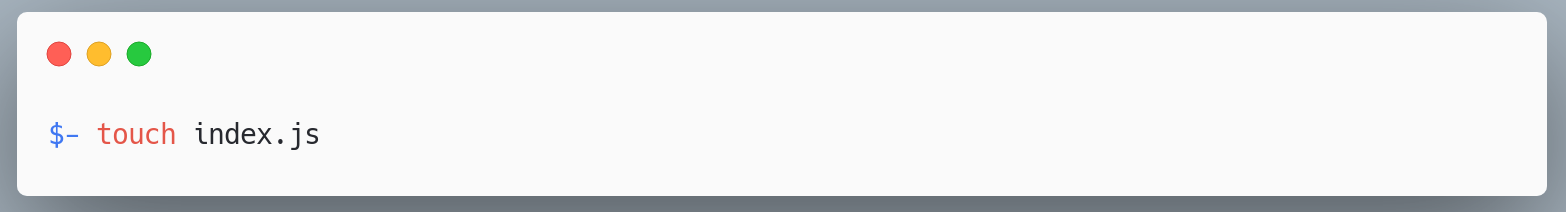
\includegraphics[width=1\textwidth]{./Imagenes/carbon.png}
    \caption[Inicializar archivo vacío]{Inicializar archivo vacío}
    \end{figure}
\newline
\newline
Dentro de este archivo debemos poner el llamado a cada elemento que se vaya agregando a nuestra librería ( Botones, Campos de texto, Tablas etc.), en la siguiente ilustración se muestra la manera en que se deben agregar los elementos.
\newline
\newline
\begin{figure}[H]
    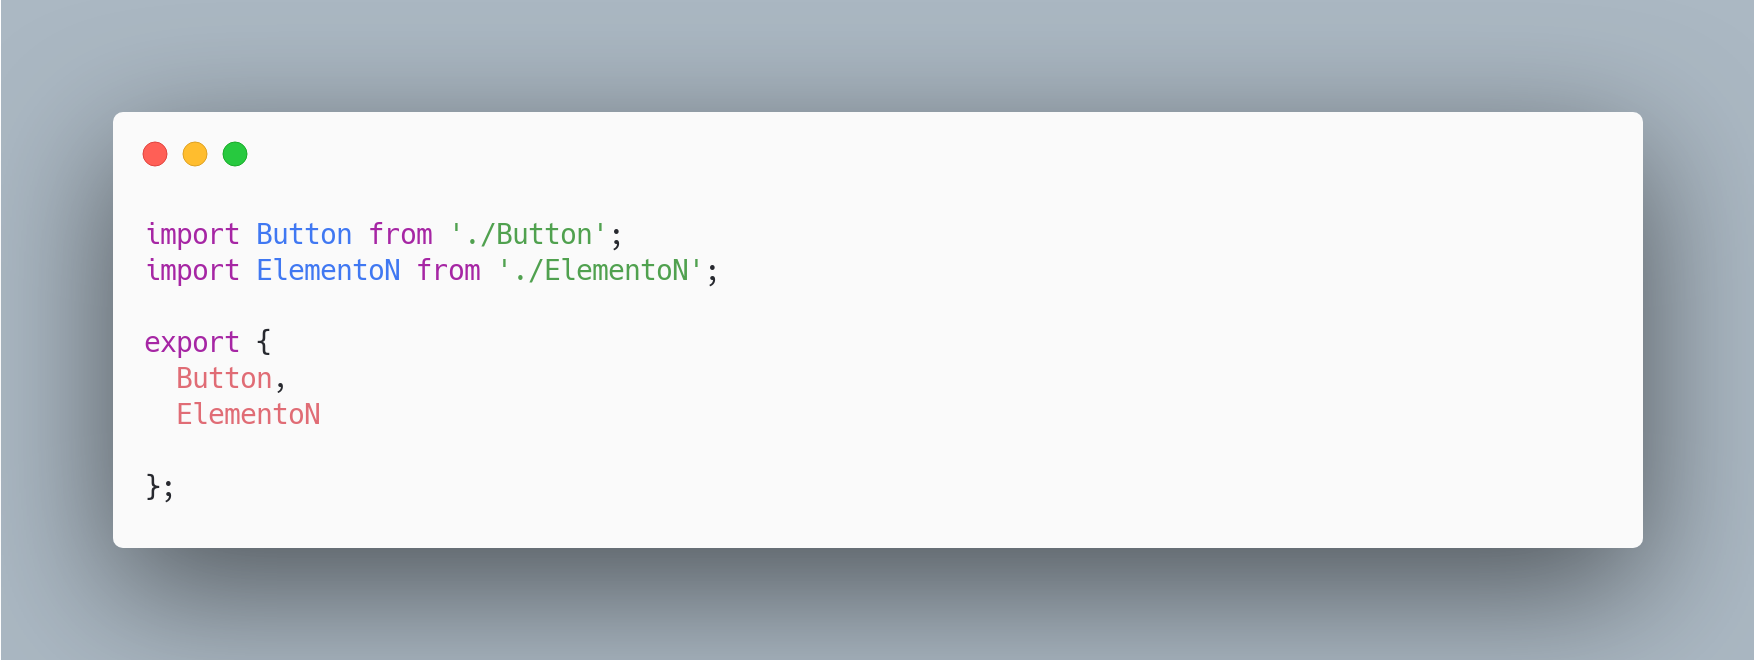
\includegraphics[width=1\textwidth]{./Imagenes/carbon-2.png}
    \caption[Inclusión de los elementos]{Inclusión de los elementos}
    \end{figure}
\newline
\newline
El primer bloque de código muestra la importación de cada uno de los elementos a nuestro archivo index, y la segunda parte exportamos un objeto de JAVASCRIPT con cada uno de los elementos.
Webpack analiza cada elemento que se incluye en el objeto y busca el contenido existente dentro de cada uno.
Cada uno de los elementos que se necesita agregar deben estar situados a la misma altura del archivo “index.js” esto dentro del directorio “src” para que puedan ser procesados.
\clearpage


\subsection{Elemento Botón}
El primer elemento que vamos a agregar es el botón, para esto creamos un directorio llamado “Botton” de la siguiente manera.
\newline
\newline
\begin{figure}[H]
    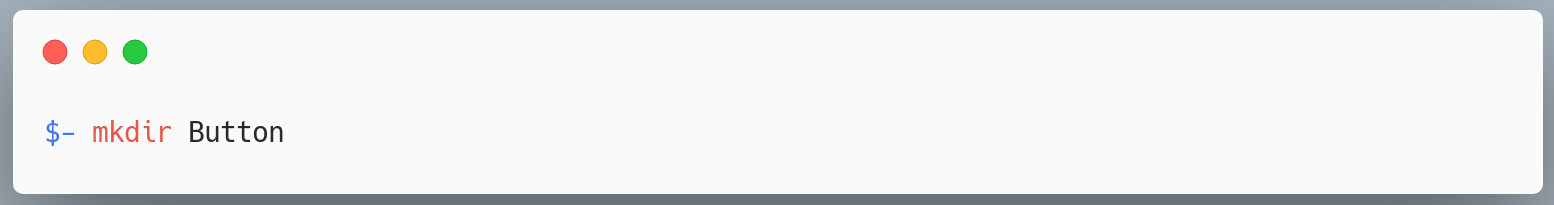
\includegraphics[width=1\textwidth]{./Imagenes/carbon-3.png}
    \caption[Crear directorio para el elemento Button]{Crear directorio para el elemento Button}
    \end{figure}
\newline
\newline
Y dentro de este directorio crearemos dos archivo que son los que incluirán el núcleo de nuestro botón, el primer archivo se llamará “index.js ” esto es así ya que por defecto, cuando importas un archivo que está dentro de un directorio, JavaScript toma el que es llamado “index.js” y no es necesario especificar este dato, esto lo podemos ver de manera clara en el archivo inicial “index.js” que está al mismo nivel que el directorio “Botton”, el cual importa el elemento Botton pero no especifica el archivo. Este archivo solamente hace el llamado al segundo archivo “Button.js” que es el que tiene el código fuente del botón. 
\newline
\newline
\begin{figure}[H]
    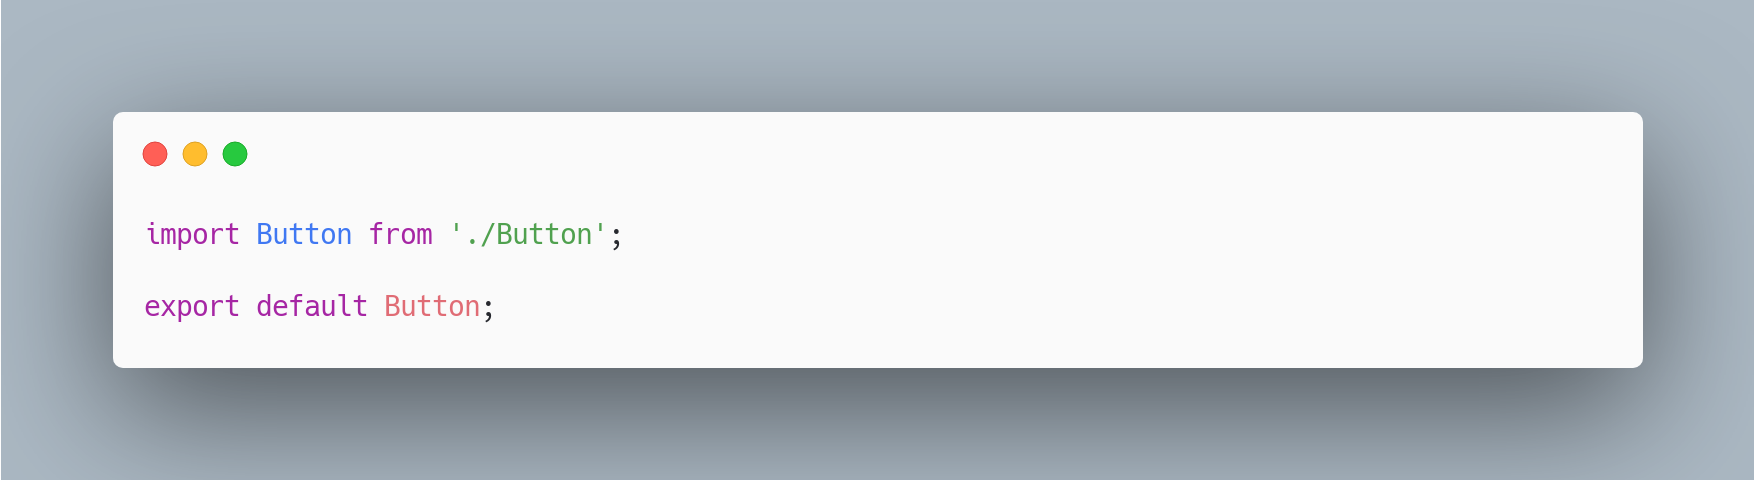
\includegraphics[width=1\textwidth]{./Imagenes/carbon-5.png}
    \caption[Contenido del elemento Button]{Contenido del elemento Button}
    \end{figure}
\newline
\newline
El segundo archivo ya mencionado “Botton.js”  hace el render de nuestro botón, y gestiona la configuración que el usuario final quiera asignarle.
En la siguiente tabla se muestran los parámetros del botón.
\newline
\newline
\begin{center}
 \begin{tabular}{ | c |  p{5cm}  | c | p{3cm} |} 
 \hline
 \textbf{Nombre} &  \textbf{Uso} &  \textbf{ Tipo de dato} &  \textbf{Valor por defecto}\\ [0.5ex] 
 \hline\hline
text & Texto que mostrará el botón.  &  Cadena de texto. & Click me! \\  [2.5ex] 
 \hline
onClick & Es la función que ejecutará cuando se hace click. & Funcion. & Función vacía. \\[2.5ex] 
 \hline
color &  Es el color del botón. & Cadena de texto. & --blue-4 \\[3.5ex] 
 \hline
 textColor & Es el color del texto en el botón. &  Cadena de texto. & --white \\[2.5ex] 
 \hline
borderColor & Es el color del borde del botón. & Cadena de texto. & --blue-4 \\ [2.5ex] 
 \hline
 type & Es el tipo de botón. & Cadena de texto. & Default \\ [2.5ex] 
 \hline
 shape & Es la forma del botón. Estos valores agregaran una curvatura, tenemos Round y SemiRound uno mas curvo que otro. & Cadena de texto. & Round \\ [2.5ex] 
 \hline
 shadow & Especifica si el botón debe tener una sombra. & Cadena de texto. & Booleano. \\ [2.5ex] 
 \hline
\end{tabular}
\end{center}
\newline
\newline
\newline
Los tipos (type) de botones que podemos tener son los siguientes.
\begin{itemize}
\item \textbf{Default:} Es el botón que se recomienda usar como principal.
\item \textbf{Secondary:} Es recomendable usarlo si ya se usa un botón default, para cuidar la jerarquía visual.
\item \textbf{Text:} Este es un botón sin contorno, debe ser usado para acciones con poca importancia.
\end{itemize}
\newline
Los parámetros obligatorios para su funcionamiento son:
\begin{itemize}
\item \textbf{text} 
\item \textbf{onClick} 
\end{itemize}
\newline
Los colores que se usan son una constante definida por la librería ya que se considera que son cromáticamente compatibles entre ellos, este tema se abordará más adelante.
A continuación se muestra un fragmento del código que permite agregar la configuración requerida.
\newline
\newline
\begin{figure}[H]
    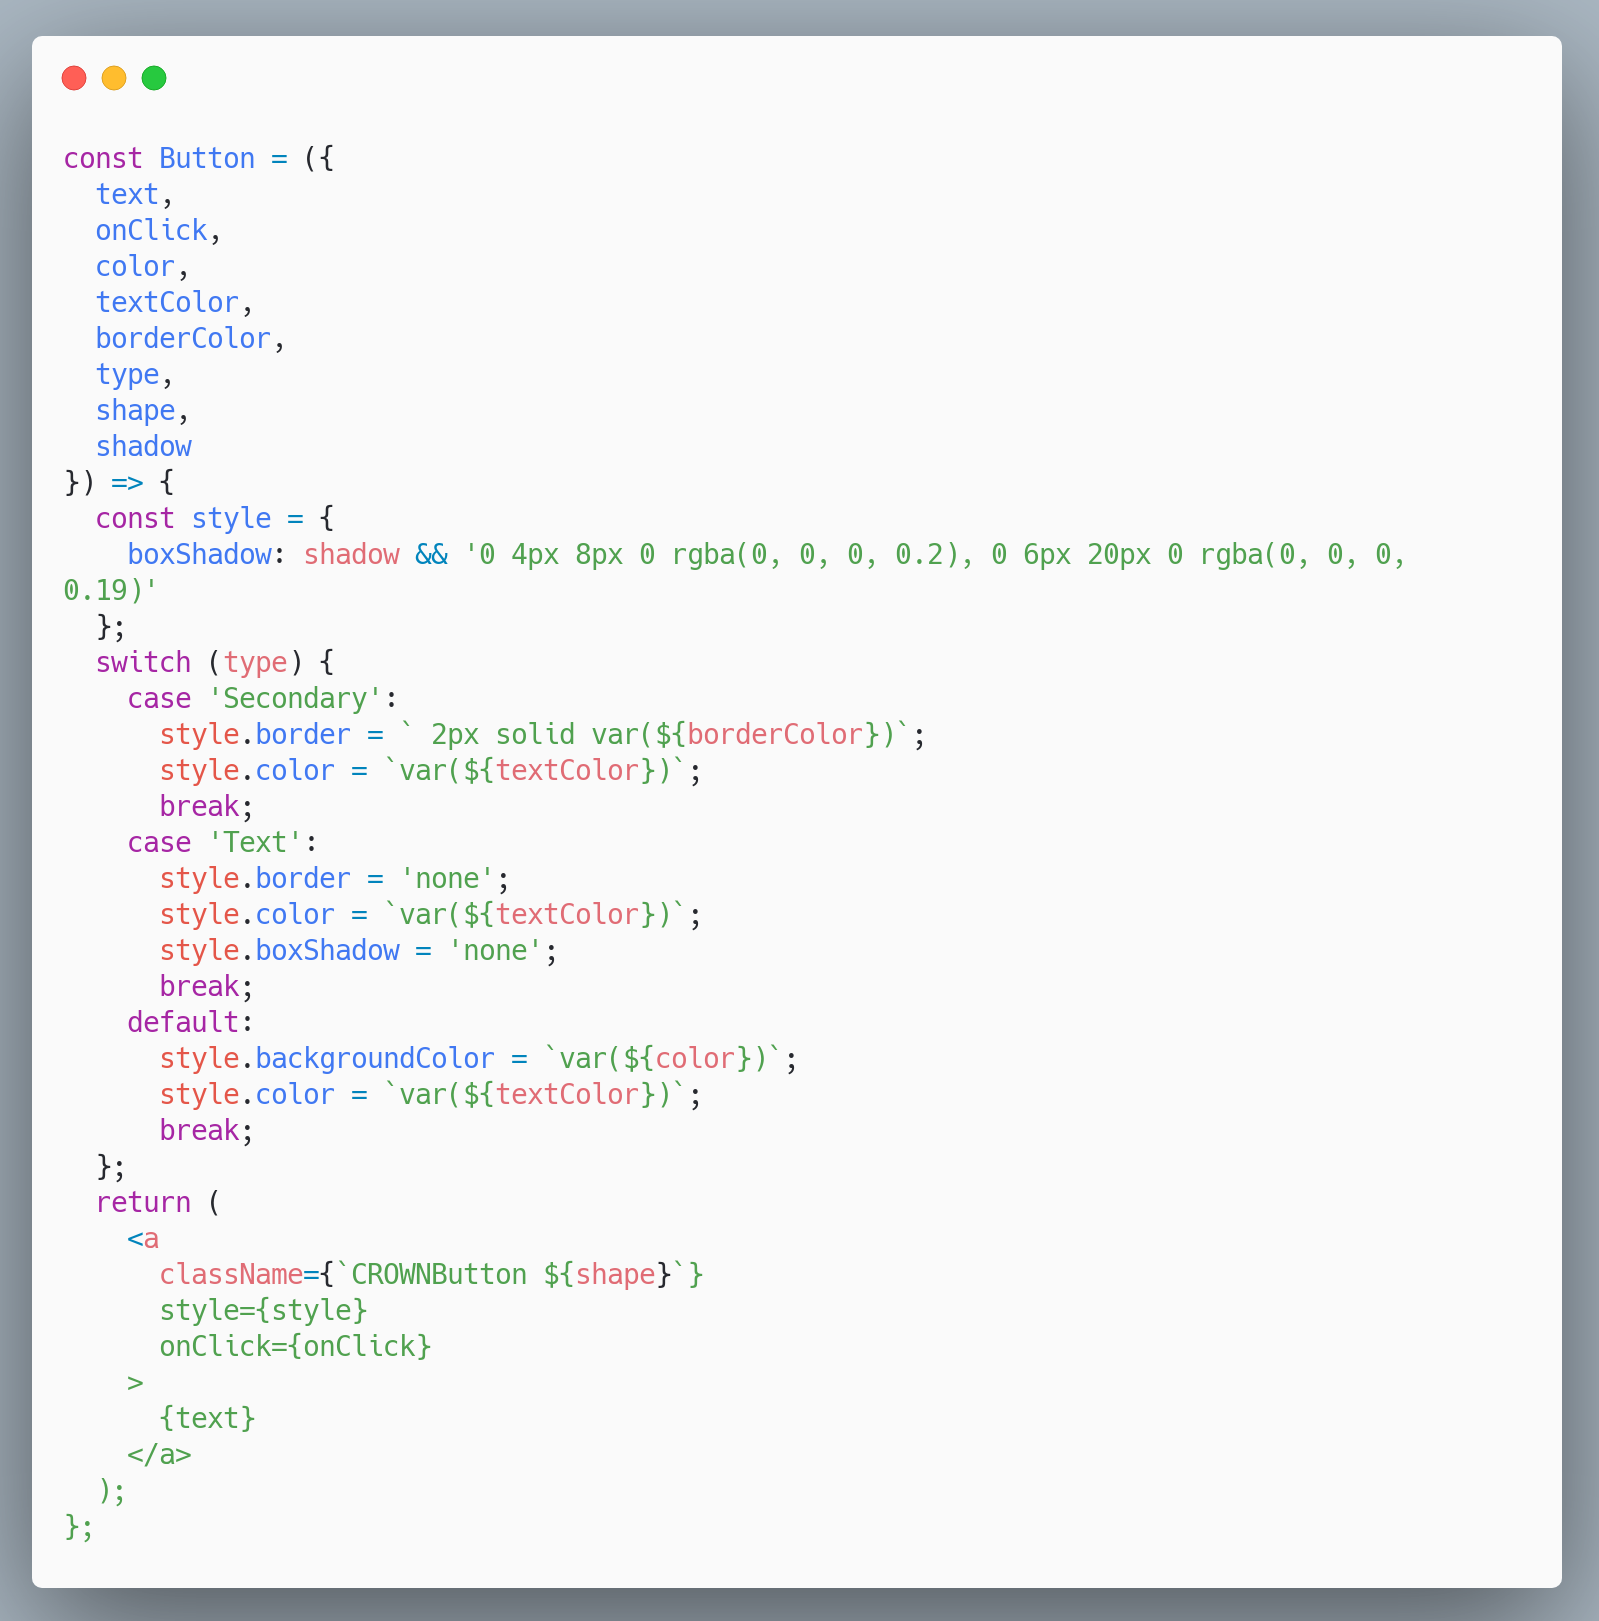
\includegraphics[width=1\textwidth]{./Imagenes/carbon-9.png}
    \caption[Código fuente del elemento Button]{Código fuente del elemento Button}
    \end{figure}
\newline
\newline
En la primera parte podemos ver una lista de la configuración dada,  después definimos un objeto llamado styles el cual agrega dentro de un switch, el css para que sea mostrado de acuerdo al tipo ( type ) de botón que se quiere. Finalmente regresa html, el cual es nuestro botón ya configurado.
Se puede observar que dentro de la etiqueta <a>  tenemos “className” esto agrega la clase en la cual definiremos el css.
Dentro del archivo css agregamos el diseño base de nuestro botón, aquí tenemos el  tamaño de la letra, tamaño del botón, grosor de letra y otras cosas más.
\newline
\newline
\begin{figure}[H]
    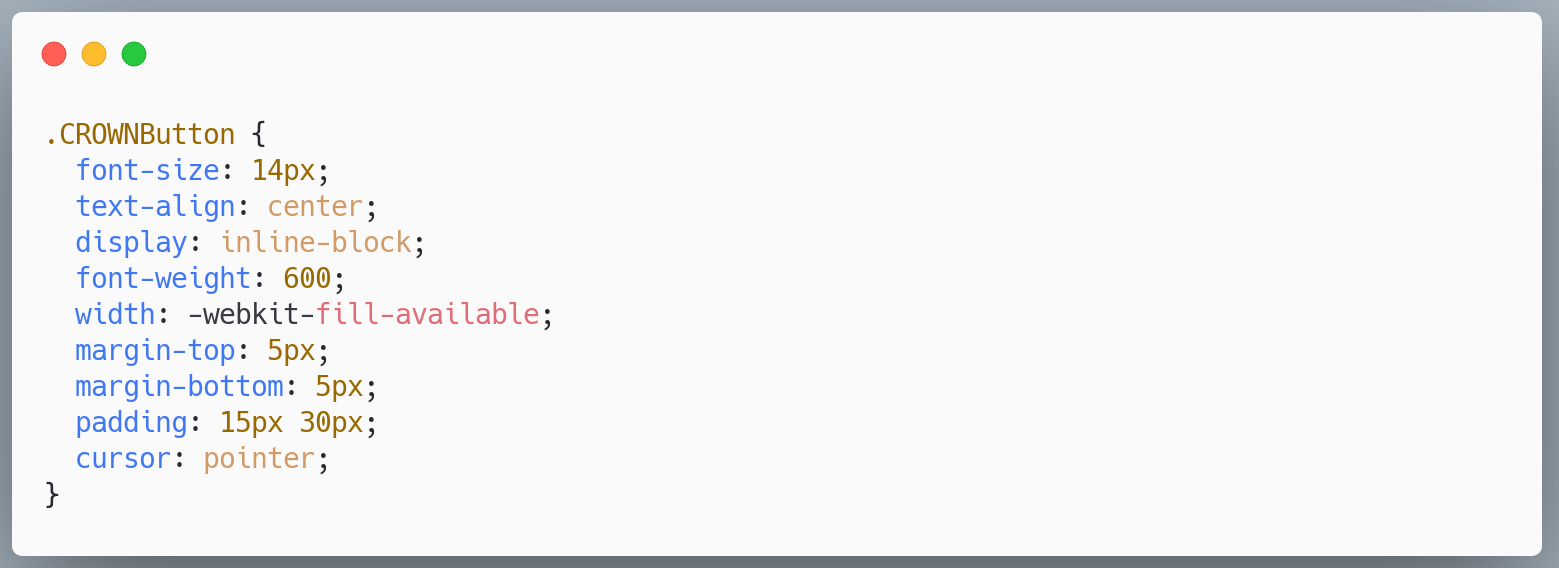
\includegraphics[width=1\textwidth]{./Imagenes/image26.png}
    \caption[Estilos del elemento Button]{Estilos del elemento Button}
    \end{figure}
\newline
\newline
\clearpage


\subsection{Elemento Label}
Ahora vamos a agregar el elemento Label que es un texto con el cual tenemos un formato estandarizado para tener un mejor diseño. En este elemento podemos dar parámetros de configuración como el tamaño, grosor y color que son los elementos básicos que se usan cuando estamos formateando con css nuestro texto. 
A continuación se presenta una lista de los parámetros y  su significado.
\newline
\begin{center}
 \begin{tabular}{ | c |  p{5cm}  | c | p{3cm} |} 
 \hline
 \textbf{Nombre} &  \textbf{Uso} &  \textbf{ Tipo de dato} &  \textbf{Valor por defecto}\\ [0.5ex] 
 \hline\hline
text 		& Este parámetro  indica el texto que vamos a mostrar.  &  Cadena de texto. 	& “I’m a label” \\  [2.5ex] 
 \hline
size 	        & Indicamos el tamaño del texto. Se cuenta con un conjunto de tamaños establecidos que se mencionan en el apartado de las constantes.       & Cadena de texto.  	& small \\[2.5ex] 
 \hline
color        & Es el color del texto.						    & Cadena de texto. 	& --black-0 \\[3.5ex] 
 \hline
 weight.   & Indicamos el grosor del texto. Se cuenta con un conjunto de tamaños establecidos que se mencionan en el apartado de las constantes.&  Cadena de texto. 	& regular \\[2.5ex] 
 \hline
\end{tabular}
\end{center}
\newline
\newline
Los parámetros obligatorios para su funcionamiento son:
\begin{itemize}
\item \textbf{text} 
\end{itemize}
\newline
\newline
Para el funcionamiento de la etiqueta de texto se tiene un componente de React en el cual se crea un objeto de JavaScript, se agrega la configuración del color, tamaño de texto y grosor. Finalmente se crea una etiqueta de html a la cual le damos nuestro objeto para que aplique el estilo y le ponemos el texto que se quiere mostrar.
\newline
\newline
\begin{figure}[H]
    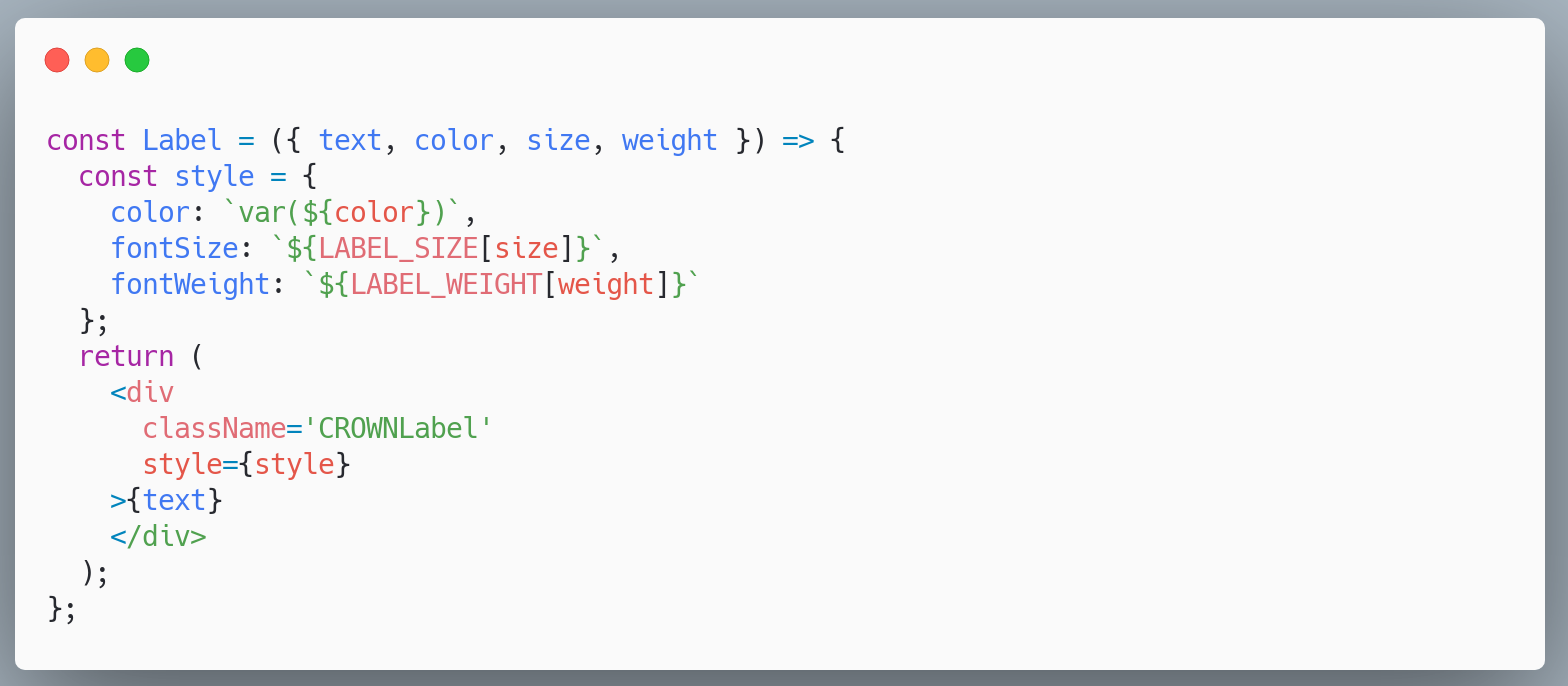
\includegraphics[width=1\textwidth]{./Imagenes/carbon-11.png}
    \caption[Código fuente del elemento Label]{Código fuente del elemento Label}
    \end{figure}
\newline
\newline
\clearpage


\subsection{Elemento Input Tex}
El input text es de utilidad para permitir la entrada de datos, y posteriormente ser procesados y enviarlos a algún servicio o procesarlos dentro de nuestra aplicación, en donde es implementado.
Los datos de entrada que son necesarios para configurar el elemento se muestran a continuación.
\newline
\newline
\begin{center}
 \begin{tabular}{ | c |  p{5cm}  | c | p{3cm} |} 
 \hline
 \textbf{Nombre} &  \textbf{Uso} &  \textbf{ Tipo de dato} &  \textbf{Valor por defecto}\\ [0.5ex] 
 \hline\hline
placeholder &Es el texto que muestra el InputText si se desea poner.  &  Cadena de texto. 	& “Write on me!” \\  [2.5ex] 
 \hline
onChange & Es la función que va a hacer invocada cuando se escriba.     & Función vacía.  	& Función vacía.l \\[2.5ex] 
 \hline
nameState & Es el nombre con el cual se identifica en el estado.    & Cadena de texto.	& input \\[3.5ex] 
 \hline
 type   & Es la manera en como será interpretado por Input Text, estos son los que existen por defecto en html. Password etc.&  Cadena de texto.	& text \\[2.5ex] 
 \hline
 title  & Si se pone como “true” este agregara un Label antes del Input Text y no lo pondrá dentro.&  Booleano.	& false \\[2.5ex] 
 \hline
 extraStyle   & Si se desea agregar más estilos se puede poner el nombre de la clase css para poder ser manipulado.&  Cadena de texto. 	& Cadena vacía. \\[2.5ex] 
 \hline
\end{tabular}
\end{center}
\newline
\newline
Los parámetros obligatorios para su funcionamiento son:
\begin{itemize}
\item \textbf{placeholder} 
\item \textbf{onChange} 
\item \textbf{nameState} 
\end{itemize}
\newline
\newline
La primera consideración que se tiene, es saber si se necesita tener un “Título” en nuestro Input Text, y si es así, se agrega un elemento Label antes,  para ayudarnos a mostrar cual es el significado de nuestro label. Esto por ejemplo, si se quiere poner una entrada de texto para solicitar el correo electronico de cierta persona, esto puede estar dentro de el Input Texto denominado placeholder o afuera denominado title, por defecto title está desactivado y se activa enviando “true”.
Cuando se escribe sobre el campo de texto, este llama a la función “onChange” que recibe, y regresa el nombre de como está identificado en el estado de REACT y el valor que contiene el campo de texto.

Los demás parámetros de los estilos también son agregados en el siguiente código.
\newline
\newline
\begin{figure}[H]
    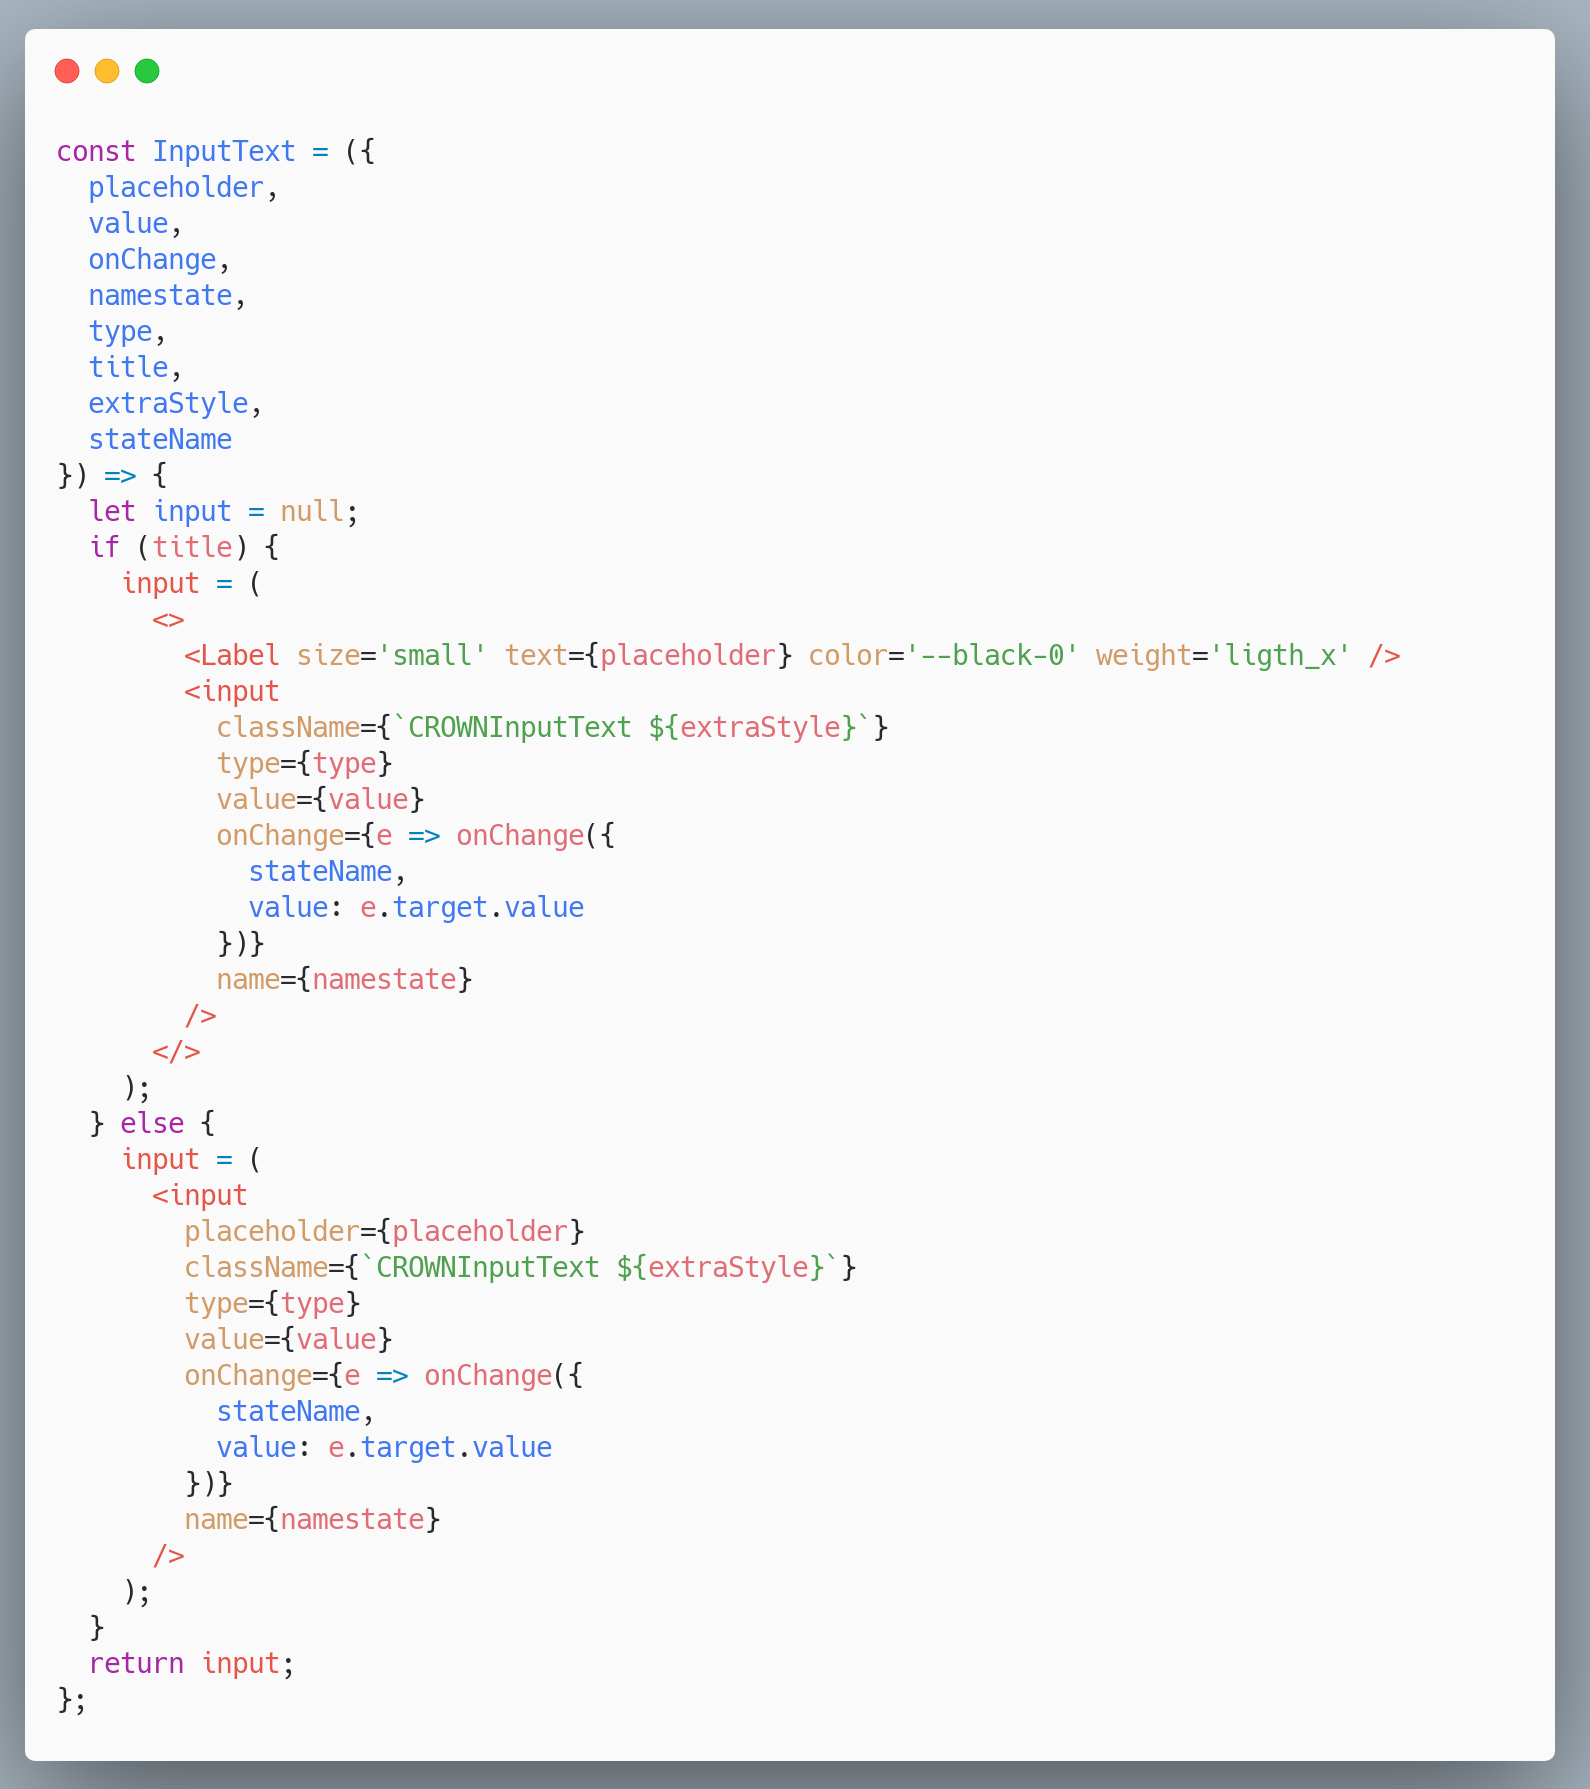
\includegraphics[width=1\textwidth]{./Imagenes/carbon-12.png}
    \caption[Código fuente del elemento InputText]{Código fuente del elemento InputText}
    \end{figure}
\newline
\newline
\clearpage


\subsection{Elemento Drop Down}
    Este elemento nos ayuda a permitir la entrada de datos, sin dar el control absoluto al momento de ingresar opciones, dada una lista en la cual es posible seleccionar una de todas. Este elemento está formado por un cuadro, que muestra la opción se encuentra activa ( al inicio ninguna ), y al hacer click se despliega el total de la lista que se recibe, dando la posibilidad de seleccionar alguna entrada.
    Los parámetros que el elemento necesita para su funcionamiento son los siguientes.
    \newline
    \newline
    \begin{center}
     \begin{tabular}{ | c |  p{5cm}  | c | p{3cm} |} 
     \hline
     \textbf{Nombre} &  \textbf{Uso} &  \textbf{ Tipo de dato} &  \textbf{Valor por defecto}\\ [0.5ex] 
     \hline\hline
     options&  Es el conjunto de las opciones para desplegar. &   Arreglo de cadenas de texto. & \\  [2.5ex] 
     \hline
     optionSelected &  Es la opción que está seleccionada actualmente. &   Cadena de texto. & \\  [2.5ex] 
     \hline
     onChange &  Es una función que se ejecutará cuando se seleccione una opción. &   Función. & Función vacía. \\  [2.5ex] 
     \hline
     stateName &  Es el nombre como es identificado en el estado de React. &  Cadena de texto & \\  [2.5ex] 
     \hline
    \end{tabular}
    \end{center}
    \newline
    \newline
Los parámetros obligatorios para su funcionamiento son:
\begin{itemize}
\item \textbf{options} 
\item \textbf{optionSelected} 
\item \textbf{onChange} 
\item \textbf{stateName} 
\end{itemize}
\newline
    \newline
    El código que se muestra a continuación es el usado para hacer funcionar nuestro elemento, el cual tiene una función que activa y desactiva las opciones de nuestro elemento cuando se hace click sobre este. La acción desencadenada modifica el estado para hacer el cambio.
    \begin{figure}[H]
    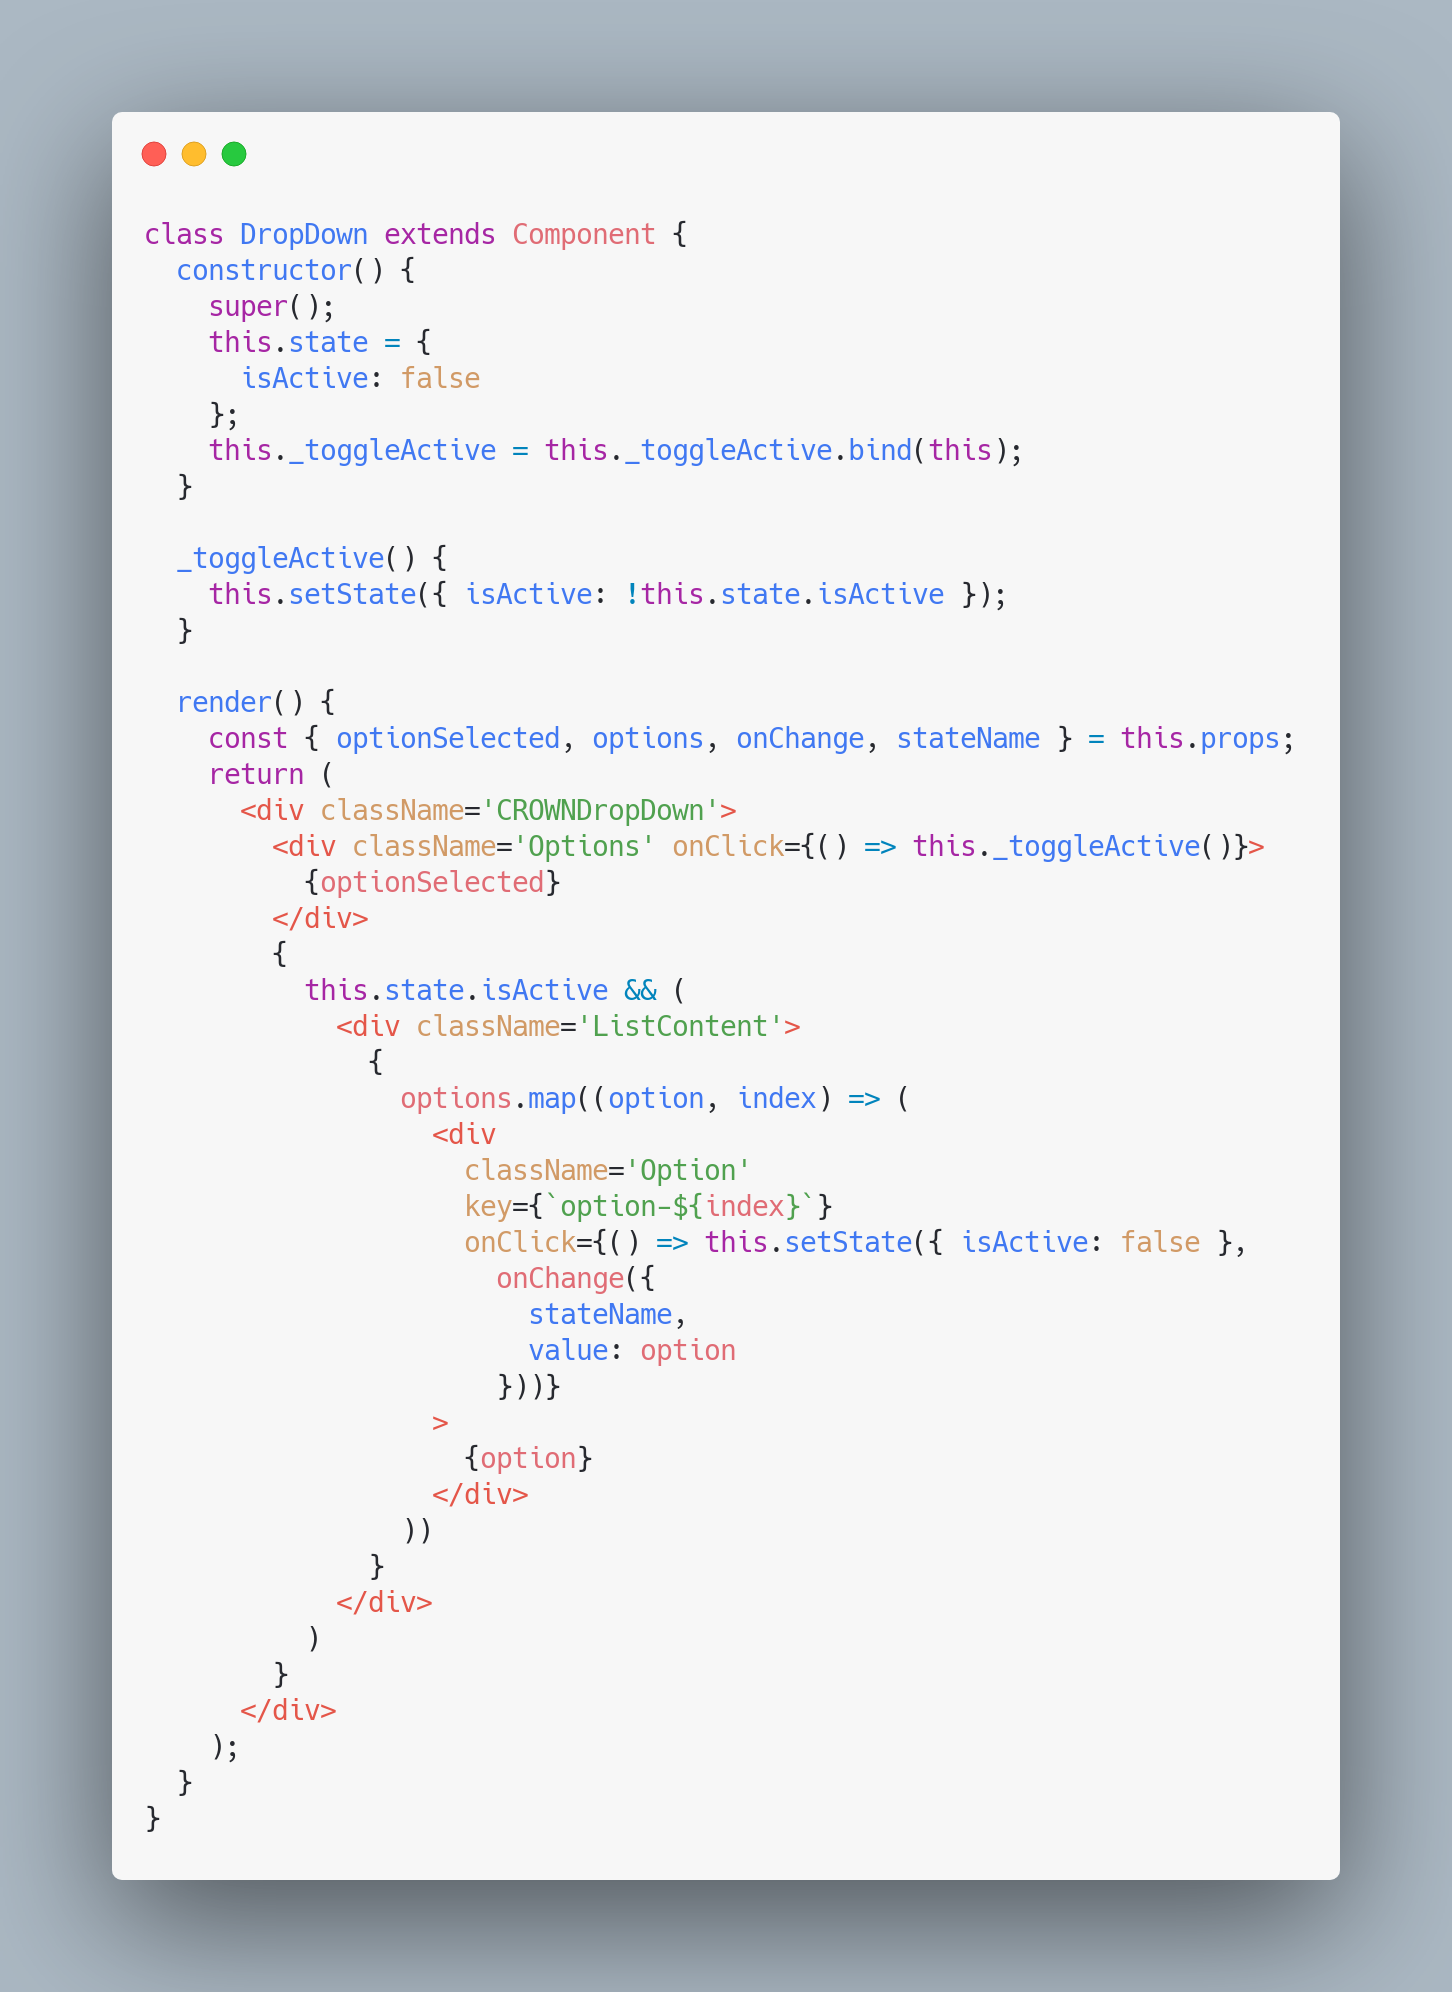
\includegraphics[width=1\textwidth]{./Imagenes/8.30.png}
    \caption[Código fuente del elemento DropDown]{Código fuente del elemento DropDown}
    \end{figure}
\clearpage


\subsection{Elemento Radio Button}
Este elemento es usado cuando se quiere dar a elegir al usuario entre un número limitado de opciones y no recomendado mayor a 3, como por ejemplo en un reactivo de un examen cuando se quiere dar a elegir si la afirmación dada es correcta o incorrecta, y las posibles respuestas es Sí o No. Este elemento solo nos permitirá a elegir una opción entre el total de respuestas.
Los parámetros que el elemento necesita para su funcionamiento son los siguientes.
  \newline
    \newline
    \begin{center}
     \begin{tabular}{ | c |  p{5cm}  | c | p{3cm} |} 
     \hline
     \textbf{Nombre} &  \textbf{Uso} &  \textbf{ Tipo de dato} &  \textbf{Valor por defecto}\\ [0.5ex] 
     \hline\hline
     options &  Son las opciones posibles a seleccionar. &   Arreglo de Objetos. & \\  [2.5ex] 
     \hline
     selectedOption &  Es la opción que está seleccionada actualmente. &   Cadena de texto. & \\  [2.5ex] 
     \hline
     onChange &  Es una función que se ejecutará cuando se seleccione una opción. &   Función. & Función vacía. \\  [2.5ex] 
     \hline
     stateName &  Es el nombre como es identificado en el estado de React. &  Cadena de texto & \\  [2.5ex] 
     \hline
    \end{tabular}
    \end{center}
    \newline
        \newline
Los parámetros obligatorios para su funcionamiento son:
\begin{itemize}
\item \textbf{options} 
\item \textbf{selectedOption} 
\item \textbf{onChange} 
\item \textbf{stateName} 
\end{itemize}
\newline
    \newline
En el siguiente código se muestra el código fuente del elemento, el cual cuando se activa una opción actualiza el estado de React
    \begin{figure}[H]
    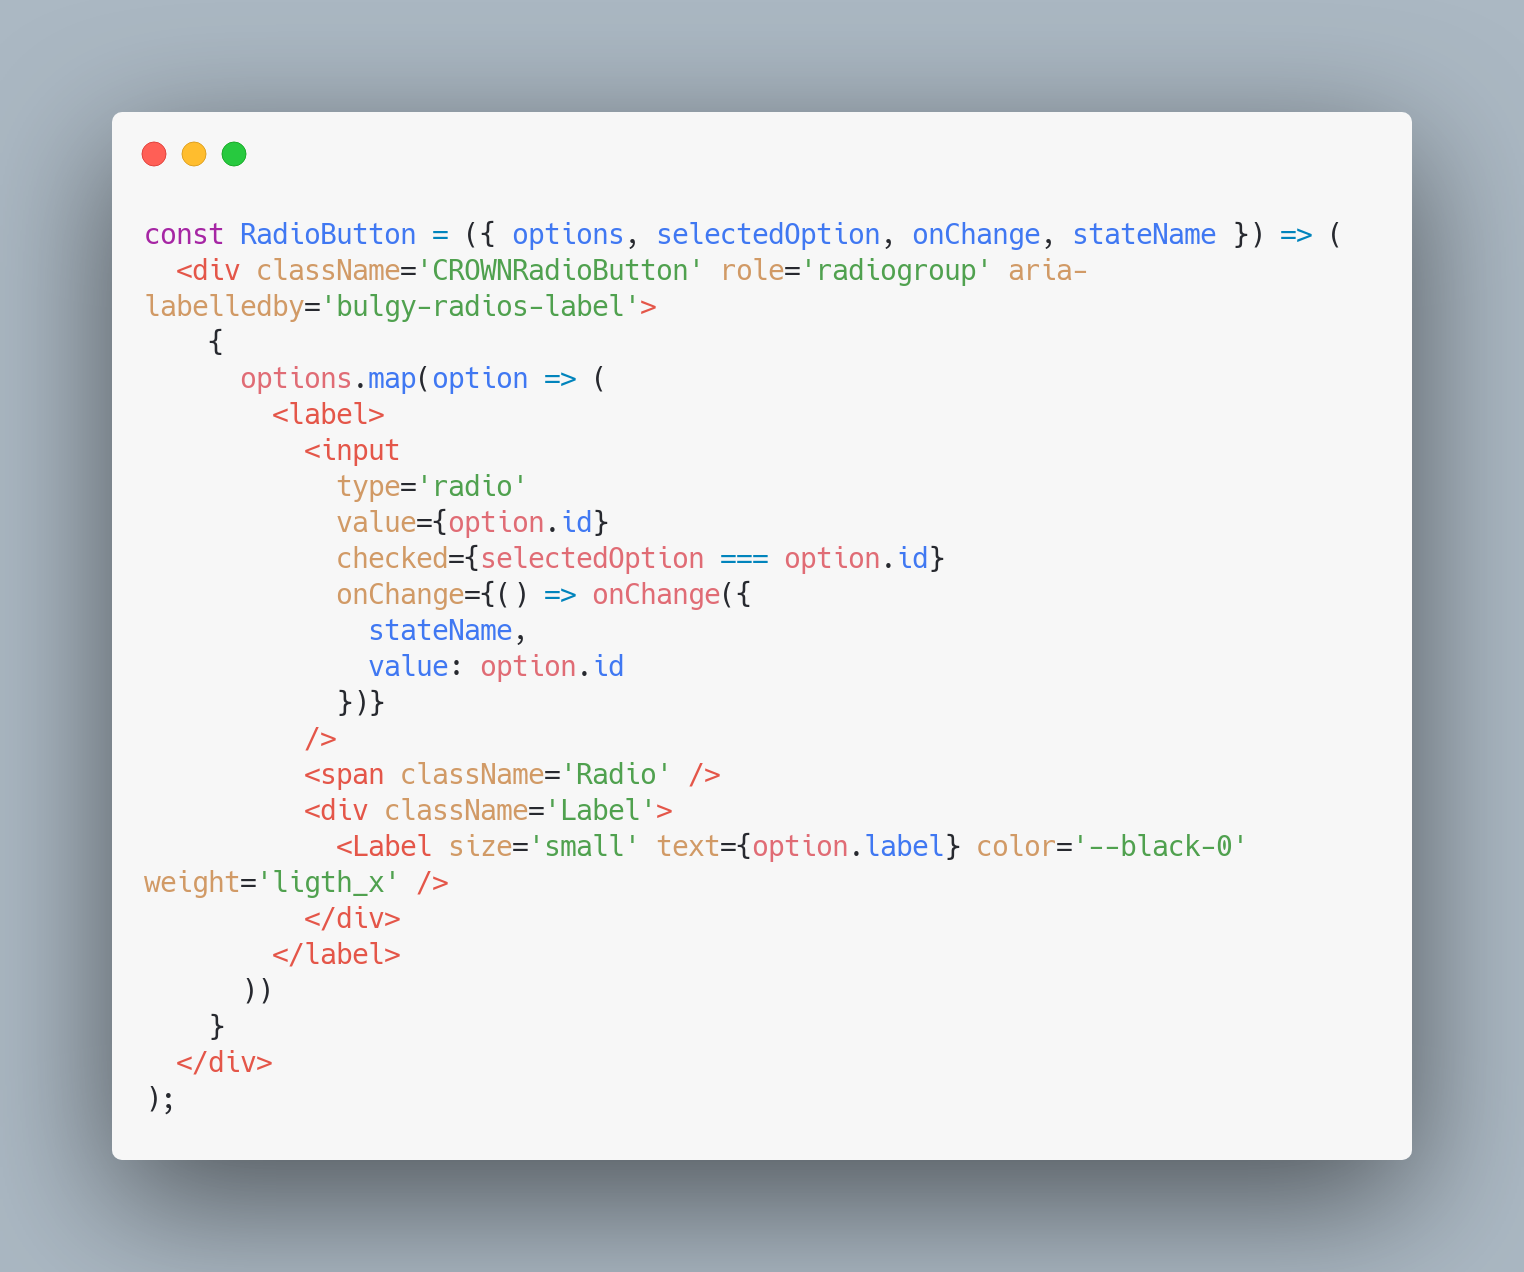
\includegraphics[width=1\textwidth]{./Imagenes/8.31.png}
    \caption[Código fuente del elemento RadioButton]{Código fuente del elemento RadioButton}
    \end{figure}
  \clearpage
  
    
    
\subsection{Elemento Switch}
Este elemento es recomendable cuando se desea iterar entre dos estados, estos son activo o inactivo. Puede ser usado, por ejemplo, cuando en una web se desea saber si el usuario quiere recibir las últimas noticias generadas.
Los parámetros que el elemento necesita para su funcionamiento son los siguientes.
\newline
    \newline
    \begin{center}
     \begin{tabular}{ | c |  p{5cm}  | c | p{3cm} |} 
     \hline
     \textbf{Nombre} &  \textbf{Uso} &  \textbf{ Tipo de dato} &  \textbf{Valor por defecto}\\ [0.5ex] 
     \hline\hline
     isChecked &  Indica si el elemento se encuentra activo o inactivo. &   Booleano. & \\  [2.5ex] 
     \hline
     onChange &  Es una función que se ejecutará cuando se seleccione una opción. &   Función. & Función vacía. \\  [2.5ex] 
     \hline
     text &  Es la etiqueta o texto que acompaña al elemento para indicar su funcionalidad. &   Cadena de texto. & Sin texto. \\  [2.5ex] 
     \hline
     stateName &  Es el nombre como es identificado en el estado de React. &  Cadena de texto. & \\  [2.5ex] 
     \hline
    \end{tabular}
    \end{center}
    \newline
        \newline
Los parámetros obligatorios para su funcionamiento son:
\begin{itemize}
\item \textbf{isChecked} 
\item \textbf{onChange} 
\item \textbf{stateName} 
\end{itemize}
\newline
    \newline
    \begin{figure}[H]
    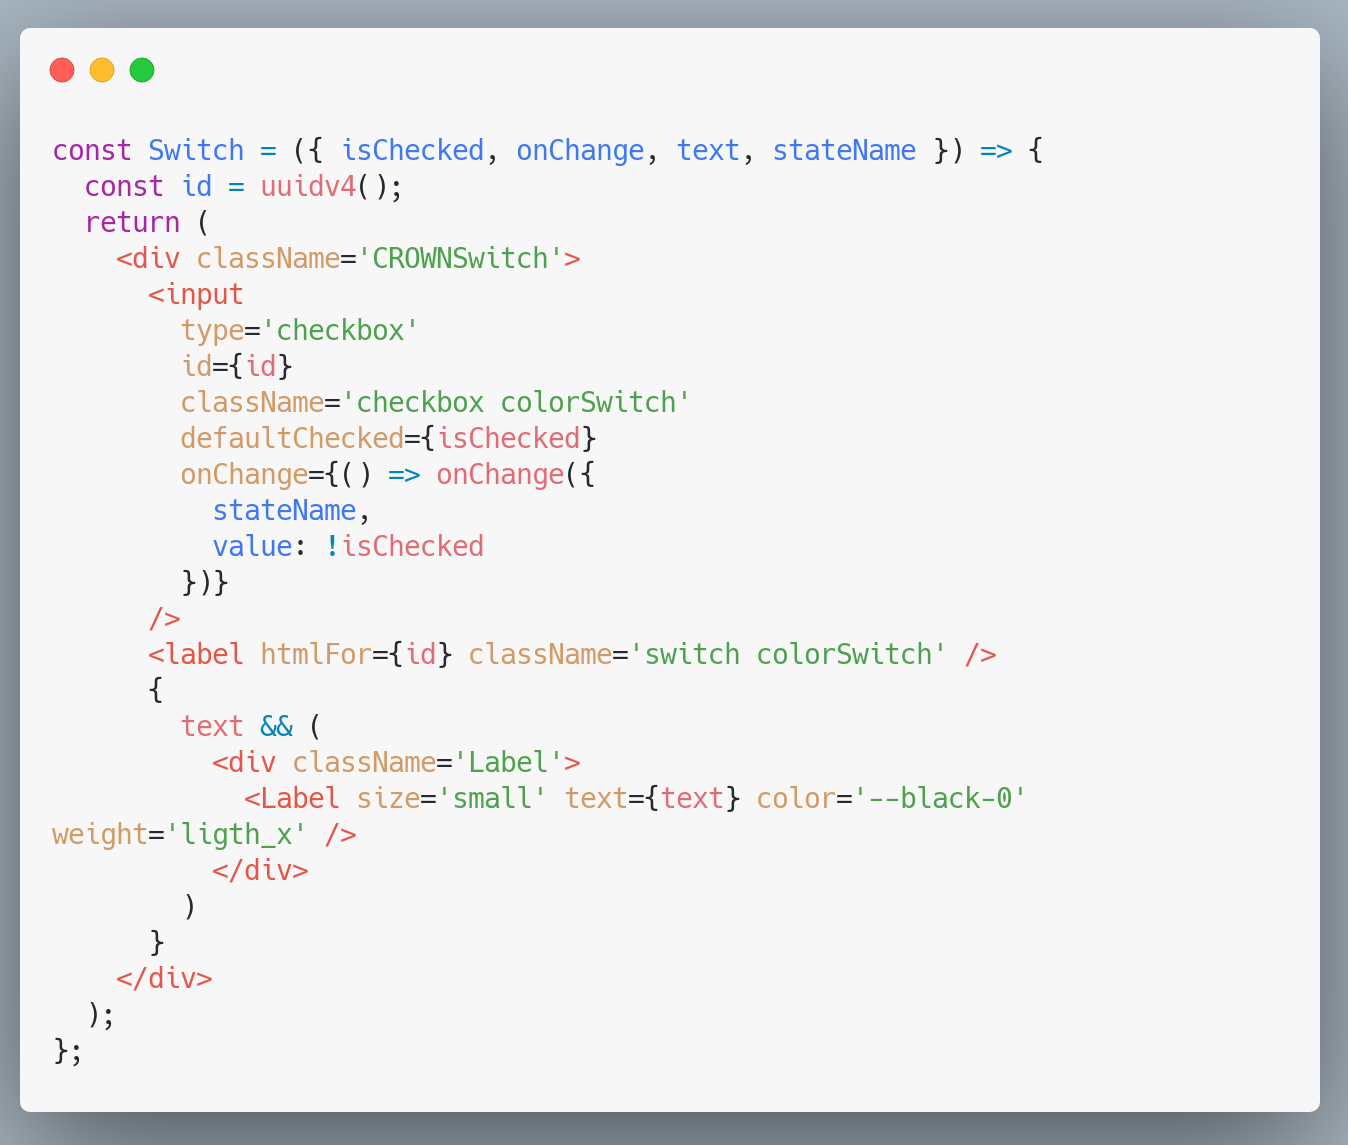
\includegraphics[width=1\textwidth]{./Imagenes/8.32.png}
    \caption[Código fuente del elemento Switch]{Código fuente del elemento Switch}
    \end{figure}
\clearpage


\subsection{Elemento Table}
Este elemento es de utilidad para mostrar datos de forma organizada como su nombre lo dice, una tabla. El elemento contiene una cabecera que indica el tipo de dato, nombre etc de la columna. También tiene el cuerpo que es en sí todos los datos.
Los parámetros que el elemento necesita para su funcionamiento son los siguientes.
\newline
    \newline
    \begin{center}
     \begin{tabular}{ | c |  p{5cm}  | c | p{3cm} |} 
     \hline
     \textbf{Nombre} &  \textbf{Uso} &  \textbf{ Tipo de dato} &  \textbf{Valor por defecto}\\ [0.5ex] 
     \hline\hline
     header &  Es el título de cada columna. &   Arreglo de cadenas. & \\  [2.5ex] 
     \hline
     body &  Es el conjunto de datos. &   Arreglo de arreglo de cadenas. & Función vacía. \\  [2.5ex] 
     \hline
    \end{tabular}
    \end{center}
    \newline
        \newline
Los parámetros obligatorios para su funcionamiento son:
\begin{itemize}
\item \textbf{body} 
\end{itemize}
\newline
    \newline
    \begin{figure}[H]
    \centering
    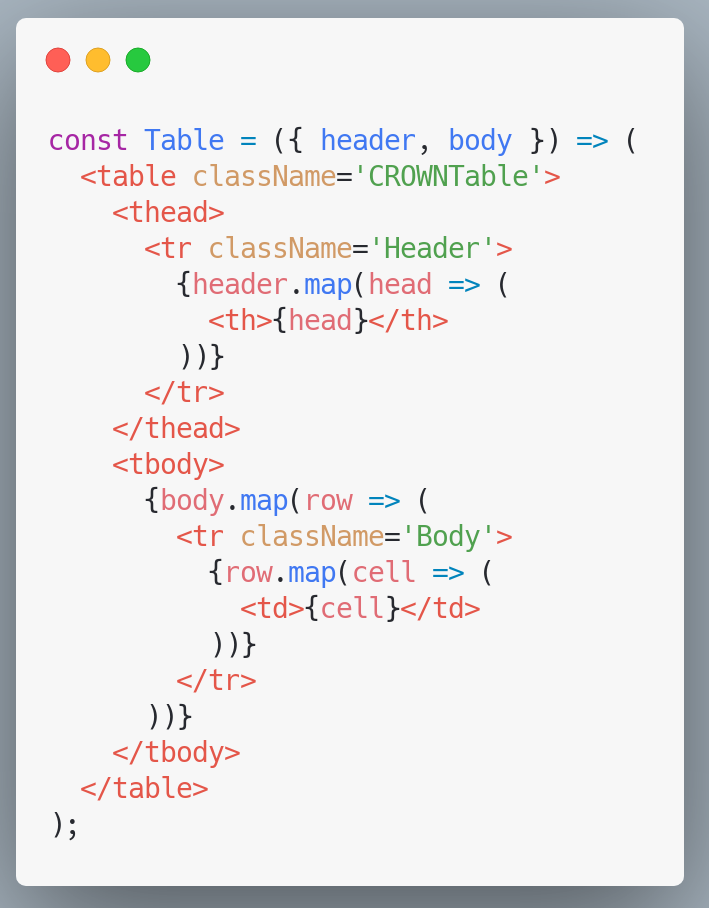
\includegraphics[width=0.5\textwidth]{./Imagenes/8.33.png}
    \caption[Código fuente del elemento Table]{Código fuente del elemento Table}
    \end{figure}
\clearpage



\subsection{Elemento CheckBox}
Este elemento es recomendable cuando se desea tener una casilla de verificación, puede ser seleccionado o sin seleccionar. Puede ser usado, por ejemplo, cuando en una web se debe forzar a aceptar los términos y condiciones para poder realizar un registro.
Los parámetros que el elemento necesita para su funcionamiento son los siguientes.
\newline
    \newline
    \begin{center}
     \begin{tabular}{ | c |  p{5cm}  | c | p{3cm} |} 
     \hline
     \textbf{Nombre} &  \textbf{Uso} &  \textbf{ Tipo de dato} &  \textbf{Valor por defecto}\\ [0.5ex] 
     \hline\hline
      isChecked & Indica si el elemento se encuentra activo o inactivo.  &  Booleano.  & \\  [2.5ex] 
     \hline
      onChange &  Es una función que se ejecutará cuando se seleccione una opción.  & Función.   &  Función vacía.\\  [2.5ex] 
     \hline
      text &  Es la etiqueta o texto que acompaña al elemento para indicar su funcionalidad. &  Cadena de texto.  & No texto. \\  [2.5ex] 
     \hline
      stateName & Es el nombre como es identificado en el estado de React.  &  Cadena de texto.  &  \\  [2.5ex] 
     \hline
    \end{tabular}
    \end{center}
    \newline
                \newline
Los parámetros obligatorios para su funcionamiento son:
\begin{itemize}
\item \textbf{isChecked} 
\item \textbf{onChange} 
\item \textbf{stateName} 
\end{itemize}
\newline
    \newline
    \begin{figure}[H]
    \centering
    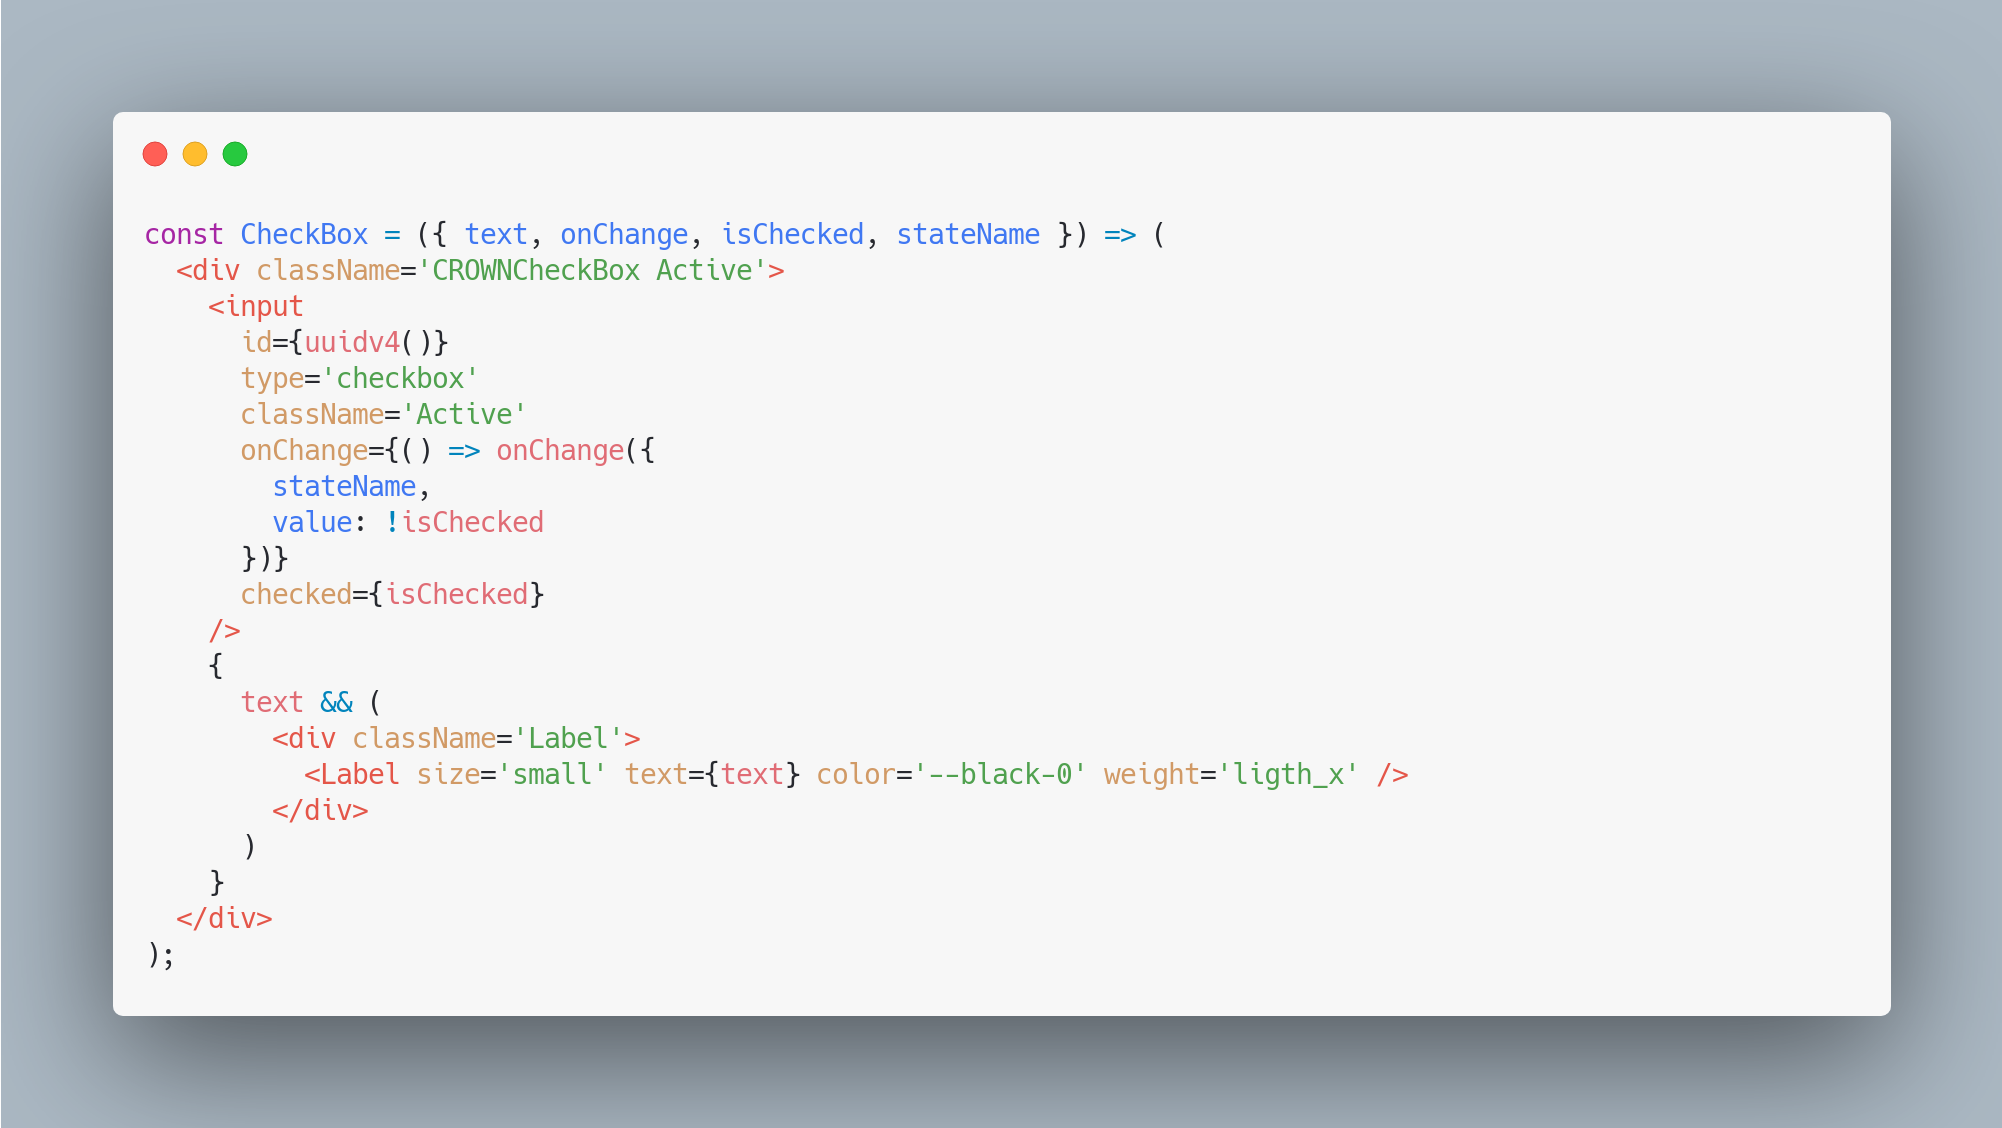
\includegraphics[width=1\textwidth]{./Imagenes/8.34.png}
    \caption[Código fuente del elemento CheckBox]{Código fuente del elemento CheckBox}
    \end{figure}
\clearpage



\subsection{Elemento Image}
Este elemento es de utilidad para agregar una imagen, en el cual solo basta con darle la dirección donde se encuentra ubicada y la librería agrega los estilos necesarios para hacer la imagen lucir.
Los parámetros que el elemento necesita para su funcionamiento son los siguientes.
\newline
    \newline
    \begin{center}
     \begin{tabular}{ | c |  p{5cm}  | c | p{3cm} |} 
     \hline
     \textbf{Nombre} &  \textbf{Uso} &  \textbf{ Tipo de dato} &  \textbf{Valor por defecto}\\ [0.5ex] 
     \hline\hline
     src &  Es la ubicación de la imagen. &   Cadena de texto. & \\  [2.5ex] 
     \hline
     frame &  Es un cuadro que se agregara al contorno de la imagen con un efecto difuminado. &   Booleano. & true \\  [2.5ex] 
     \hline
      shadow &  Es una sombra al contorno de la imagen. &   Booleano. & true \\  [2.5ex] 
     \hline
     size &  Es el tamaño en pixeles de la imagen. &   Arreglo de arreglo de cadenas. & Objeto. \\  [2.5ex] 
     \hline
    \end{tabular}
    \end{center}
    \newline
                \newline
Los parámetros obligatorios para su funcionamiento son:
\begin{itemize}
\item \textbf{src} 
\end{itemize}
\newline
    \newline
    \begin{figure}[H]
    \centering
    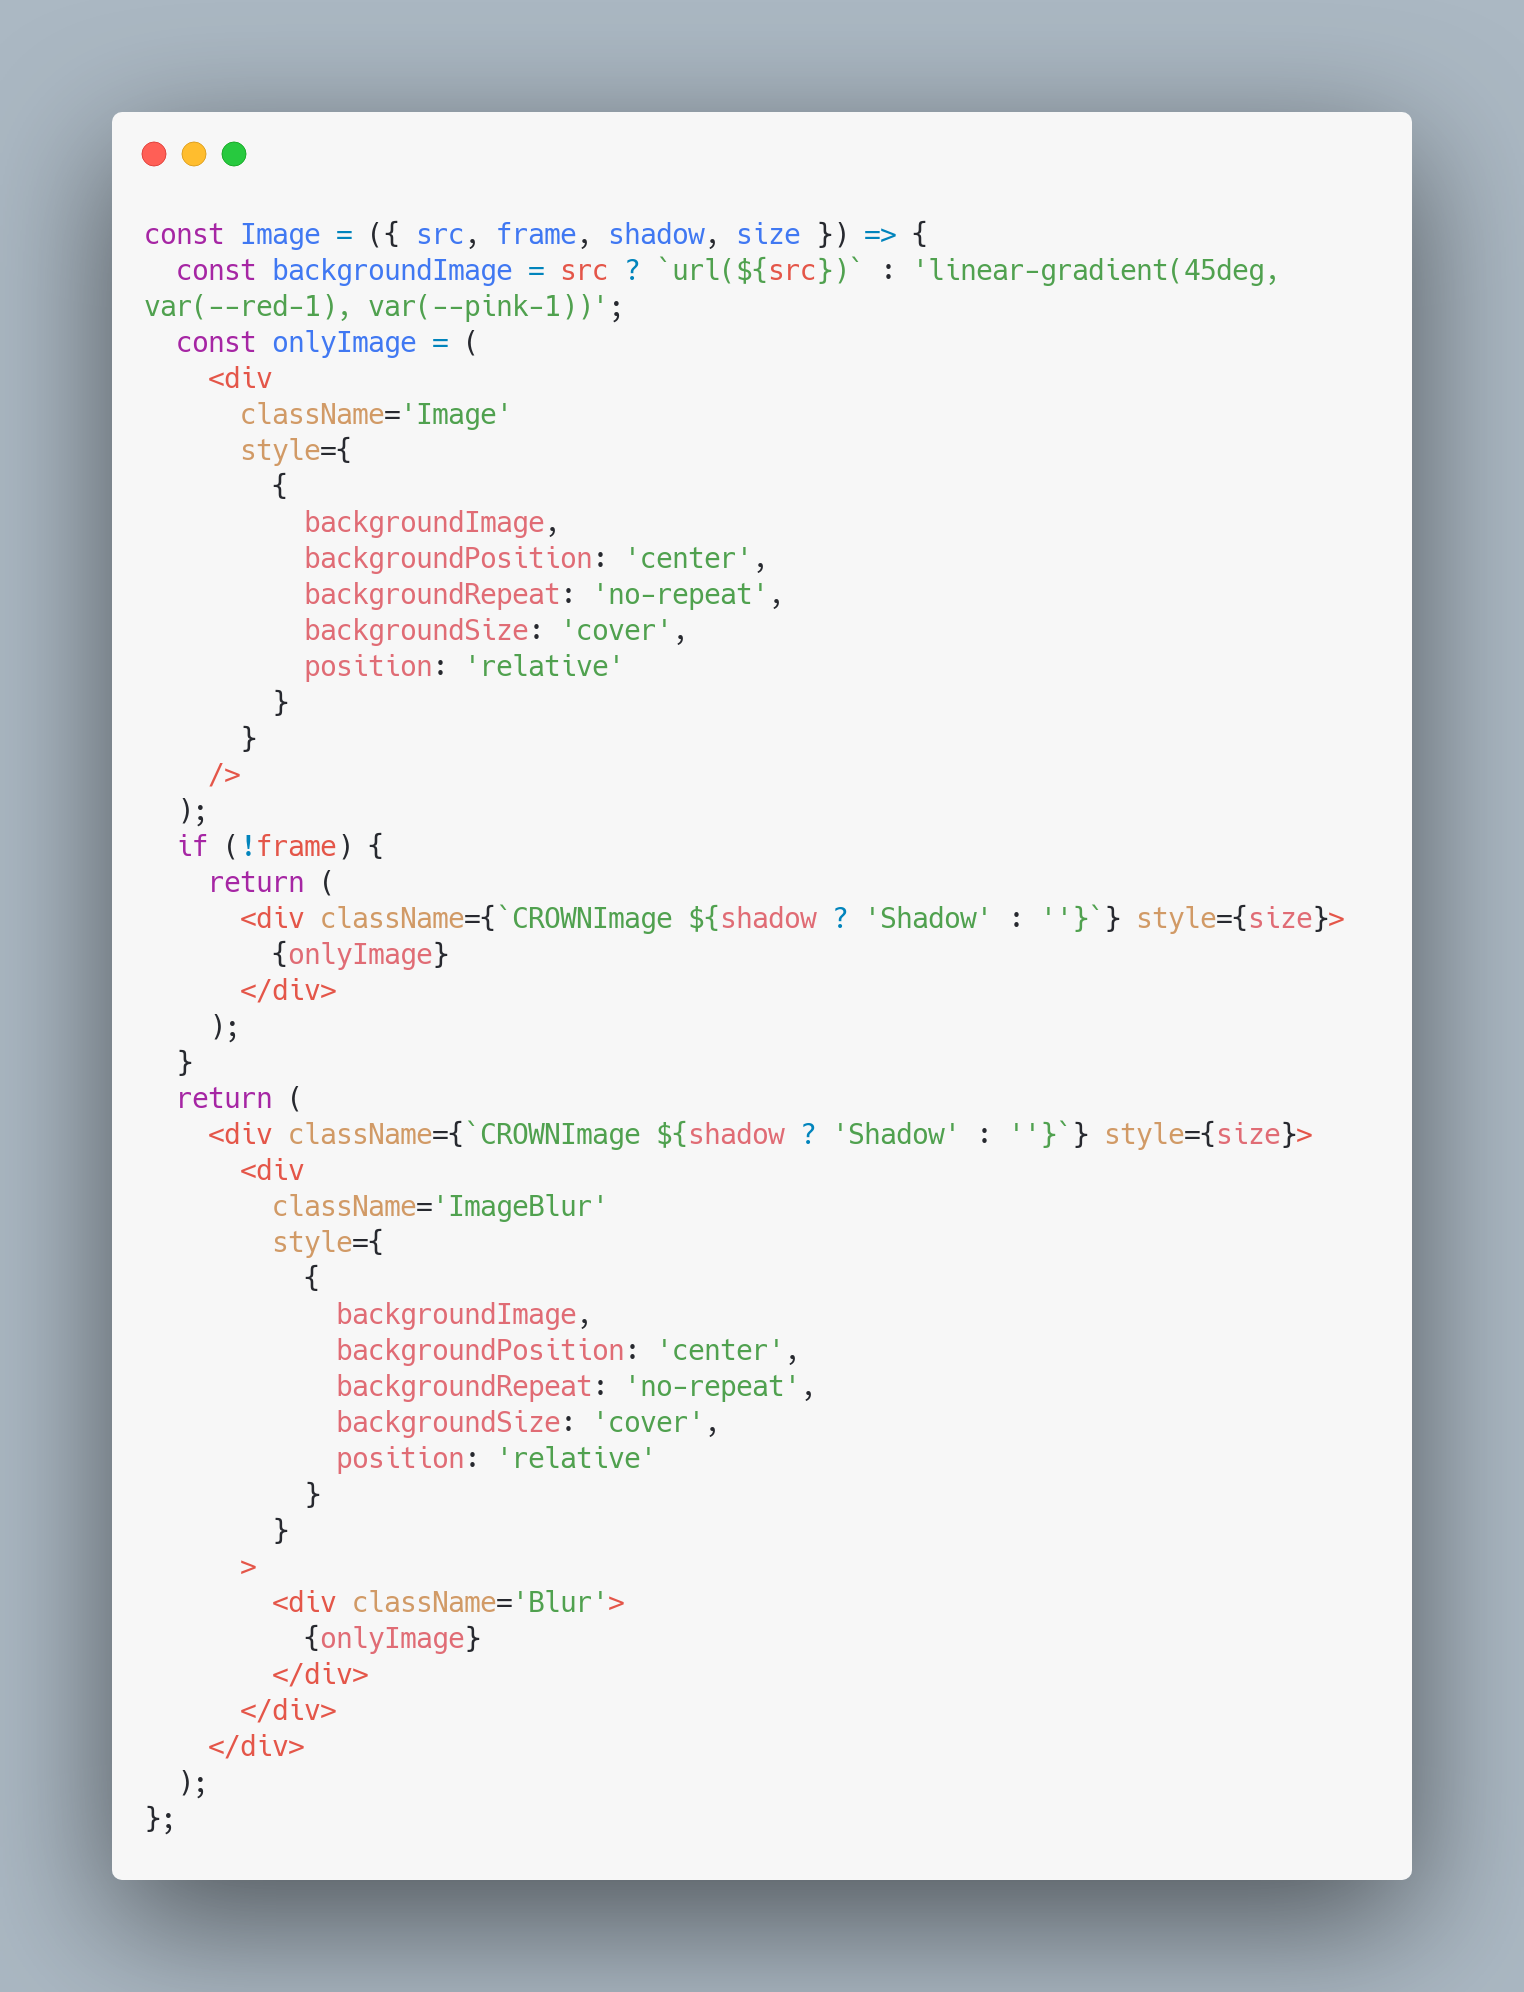
\includegraphics[width=1\textwidth]{./Imagenes/8.35.png}
    \caption[Código fuente del elemento Image]{Código fuente del elemento Image}
    \end{figure}
   \clearpage
   
    
    
    \subsection{Elemento Loader}
Este elemento se recomienda usar cuando se desea dar la retroalimentación al usuario, cuando se están ejecutando procesos de la aplicación y es necesario esperar a que estos terminen para poder avanzar.
Con la presente librería es relativamente simple hacer la implementación.

El parámetro que el elemento necesita para su funcionamiento es.
\newline
    \newline
    \begin{center}
     \begin{tabular}{ | c |  p{5cm}  | c | p{3cm} |} 
     \hline
     \textbf{Nombre} &  \textbf{Uso} &  \textbf{ Tipo de dato} &  \textbf{Valor por defecto}\\ [0.5ex] 
     \hline\hline
     show &  Indicar si el elemento debe mostrarse. &   Booleano. &  false \\  [2.5ex] 
     \hline
    \end{tabular}
    \end{center}
    \newline
                \newline
Los parámetros obligatorios para su funcionamiento son:
\begin{itemize}
\item \textbf{show} 
\end{itemize}
\newline
    \newline
    \begin{figure}[H]
    \centering
    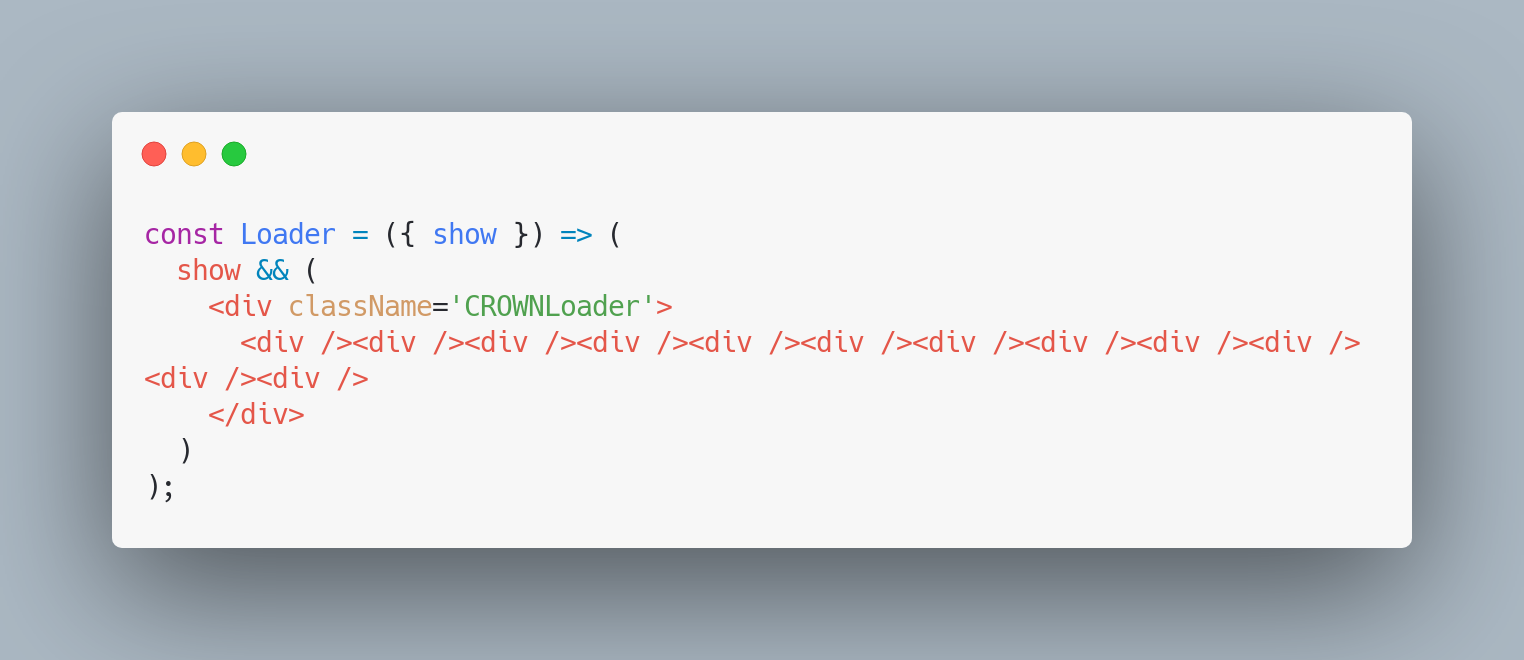
\includegraphics[width=1\textwidth]{./Imagenes/8.36.png}
    \caption[Código fuente del elemento Image]{Código fuente del elemento Image}
    \end{figure}
\clearpage


    \subsection{Elemento Card}
    Este elemento se usa cuando queremos mostrar tarjetas de información, las cuales contienen imagen, texto y botones. Por ejemplo si se desea desarrollar una web para un restaurante podemos implementar este elemento el cual nos facilitará la tarea, porque podemos darle la imagen del restaurante o algún platillo que se quisiera mostrar, también le podemos dar la descripción, título y un botón que realizará una acción con cada tarjeta.
Los parámetros que el elemento necesita para su funcionamiento son los siguientes.
\newline
    \newline
    \begin{center}
     \begin{tabular}{ | c |  p{5cm}  | c | p{3cm} |} 
     \hline
     \textbf{Nombre} &  \textbf{Uso} &  \textbf{ Tipo de dato} &  \textbf{Valor por defecto}\\ [0.5ex] 
     \hline\hline
     src &  Imagen a mostrar. &   Cadena de texto. &  false \\  [2.5ex] 
     \hline
      title & Título de la tarjeta. &   Cadena de texto. &  Card Title \\  [2.5ex] 
     \hline
     content & Contenido de la tarjeta. &   Cadena de texto. &  Card Content  \\  [2.5ex] 
     \hline
     buttonConfig &  Configuración del botón. &   Objeto. &  false \\  [2.5ex] 
     \hline
     customButton &  Elemento Button previamente configurado. &   Componente. &  false \\  [2.5ex] 
     \hline
    \end{tabular}
    \end{center}
    \newline
            \newline
Los parámetros obligatorios para su funcionamiento son:
\begin{itemize}
\item \textbf{content} 
\item \textbf{buttonConfig} 
\end{itemize}
\newline
    \newline
    \begin{figure}[H]
    \centering
    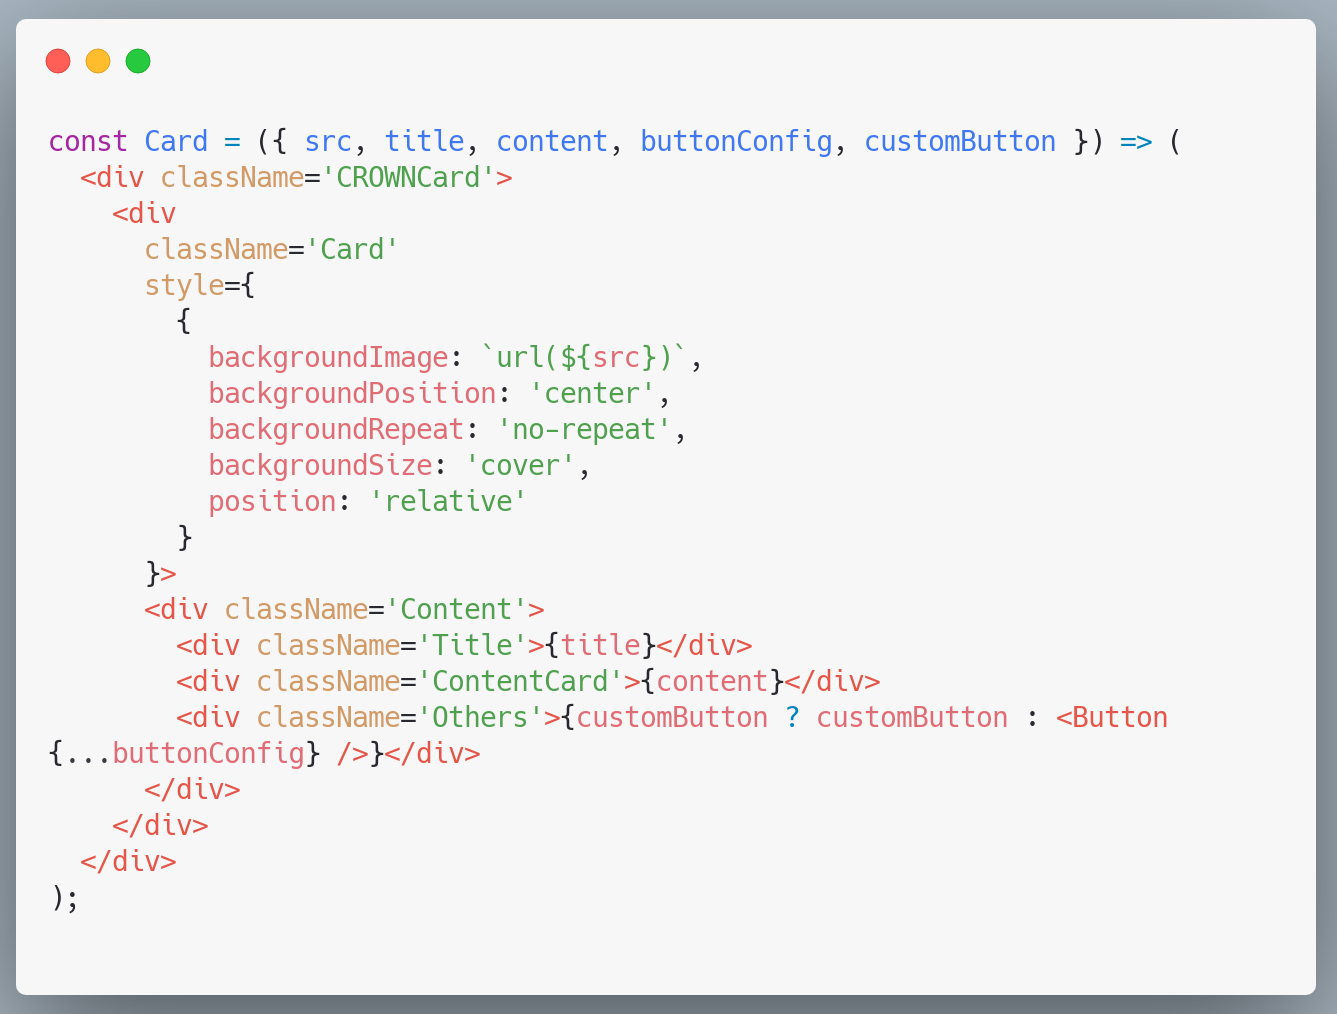
\includegraphics[width=1\textwidth]{./Imagenes/8.37.png}
    \caption[Código fuente del elemento Card]{Código fuente del elemento Card}
    \end{figure}
\clearpage





    \subsection{Elemento Modal}
    Este elemento es crucial para alertar de una acción la cual requiere de una mayor precaución. Por ejemplo un botón que al presionar ejecuta un proceso el cual elimina algún registro de la base de datos permanentemente.
Con este podemos mandar un mensaje de advertencia el cual confirmará o denegará  la acción, y luego el flujo continuará habitualmente.
Los parámetros que el elemento necesita para su funcionamiento son los siguientes.
\newline
    \newline
    \begin{center}
     \begin{tabular}{ | c |  p{5cm}  | c | p{3cm} |} 
     \hline
     \textbf{Nombre} &  \textbf{Uso} &  \textbf{ Tipo de dato} &  \textbf{Valor por defecto}\\ [0.5ex] 
     \hline\hline
      show &  Indicar si el elemento debe mostrarse. &  Booleano. &  false. \\  [2.5ex] 
      \hline
      onClose &   Acción a realizar si el modal se cierra. &  Función.  &  Función vacía. \\  [2.5ex] 
      \hline
      onActionAcepted &   Acción a realizar si se acepta la acción. &  Función.  &  Función vacía. \\  [2.5ex] 
      \hline
      onActionRejected &  Acción a realizar si se deniega la acción. & Función.  &  Función vacía. \\  [2.5ex] 
      \hline
      child &  Contenido para un modal personalizado.  & Componente de React.  &  Nulo \\  [2.5ex] 
      \hline
      title &   Título del modal. & Cadena de texto.   &  Modal Title  \\  [2.5ex] 
      \hline
      content&  Contenido del modal.  &  Cadena de texto.  &   Content Title\\  [2.5ex] 
     \hline
    \end{tabular}
    \end{center}
    \newline
        \newline
Los parámetros obligatorios para su funcionamiento son:
\begin{itemize}
\item \textbf{show} 
\item \textbf{onClose} 
\item \textbf{onChange} 
\item \textbf{onActionAcepted} 
\item \textbf{onActionRejected} 
\item \textbf{content} 
\end{itemize}
\newline
    \newline
    \begin{figure}[H]
    \centering
    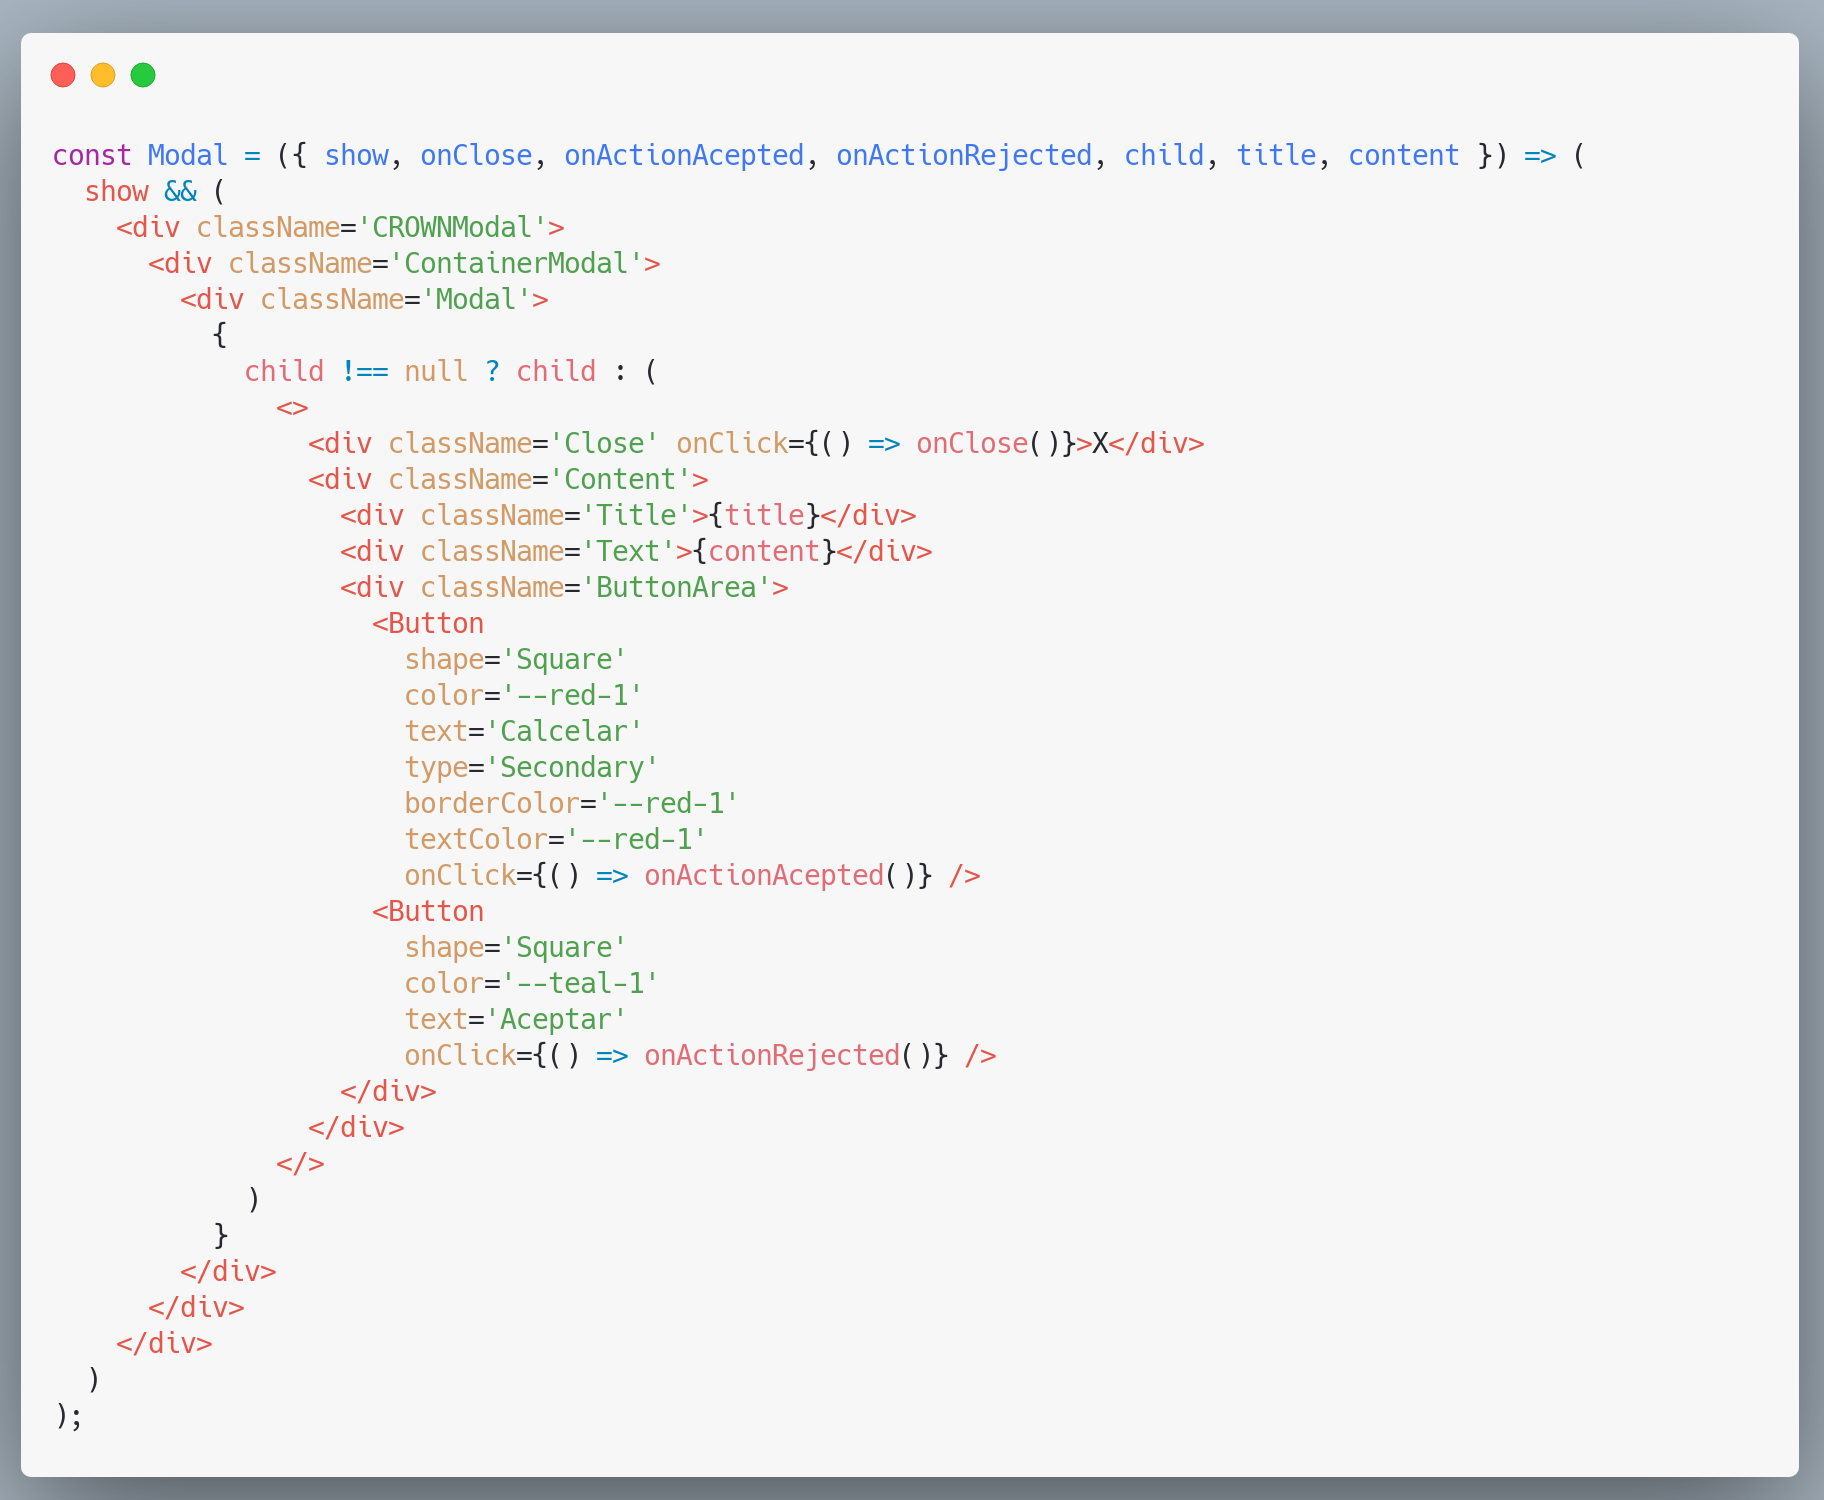
\includegraphics[width=1\textwidth]{./Imagenes/8.38.png}
    \caption[Código fuente del elemento Modal]{Código fuente del elemento Modal}
    \end{figure}
    \clearpage
